% ============================================================
%  Projective Dynamic Logo (PDL)
%  Global Mapping of Structures, Results, and Open Problems
%  Version 15  —  C. Laubscher
% ============================================================
\documentclass[11pt,a4paper]{article}

% ---- Encoding and fonts ----
\usepackage[utf8]{inputenc}
\usepackage[T1]{fontenc}

% ---- Page layout ----
\usepackage[margin=2.5cm]{geometry}

% ---- Mathematics ----
\usepackage{amsmath,amssymb,amsthm}

% ---- Tables and lists ----
\usepackage{booktabs}
\usepackage{longtable}
\usepackage{array}
\usepackage{ragged2e}
\usepackage{enumitem}
\newcolumntype{L}[1]{>{\RaggedRight\arraybackslash}p{#1}}

% ---- Graphics ----
\usepackage{graphicx}
\usepackage{float}
\usepackage{tikz}
\usetikzlibrary{positioning,backgrounds,arrows.meta,fit}

% ---- Captions and colours ----
\usepackage[font=small,labelfont=bf]{caption}
\captionsetup[table]{labelsep=quad}
\usepackage{xcolor}
\definecolor{proofblue}{RGB}{0,70,140}
\definecolor{conjecturegreen}{RGB}{0,120,60}
\definecolor{hypothesisorange}{RGB}{200,90,0}
\definecolor{openproblemred}{RGB}{170,0,0}

% ---- Hyperlinks ----
\usepackage{hyperref}
\usepackage{doi}
\usepackage{url}
\hypersetup{
  colorlinks=true,
  linkcolor=proofblue,
  citecolor=proofblue,
  urlcolor=proofblue
}

% ---- Bibliography ----
\usepackage[numbers]{natbib}

% ---- Theorem environments ----
\theoremstyle{plain}
\newtheorem{theorem}{Theorem}[section]
\newtheorem{proposition}[theorem]{Proposition}
\newtheorem{corollary}[theorem]{Corollary}
\newtheorem{lemma}[theorem]{Lemma}
\theoremstyle{definition}
\newtheorem{definition}[theorem]{Definition}
\newtheorem{axiom}[theorem]{Axiom}
\theoremstyle{remark}
\newtheorem{remark}[theorem]{Remark}
\newtheorem{conjecture}[theorem]{Conjecture}
\newtheorem{openproblem}[theorem]{Open Problem}
\newtheorem{hypothesis}[theorem]{Hypothesis}

% ---- Custom macros ----
\newcommand{\PDL}{\textnormal{PDL}}
\newcommand{\Kfour}{K_4}
\newcommand{\quintuplet}{(24,\,28,\,930,\,10087,\,11017)}
\newcommand{\Geff}{G_{\mathrm{eff}}}
\newcommand{\GPDL}{G_{\mathrm{PDL}}}
\newcommand{\epsG}{\varepsilon_G}
\newcommand{\rval}{r_{\mathrm{val}}}
\newcommand{\Rsurf}{R_{\mathrm{surf}}}
\newcommand{\Rtot}{R_{\mathrm{tot}}}
\newcommand{\sigmaN}{\sigma(N)}
\newcommand{\mustar}{\mu^*}
\newcommand{\SBH}{S_{\mathrm{BH}}}
\newcommand{\Meff}{M_{\mathrm{eff}}}
\newcommand{\MPl}{M_{\mathrm{Pl}}}
\newcommand{\Tpp}{T_{pp}}
\newcommand{\Zsat}{Z_{\mathrm{sat}}}
\newcommand{\Nmin}{N_{\min}}

% ---- List style ----
\setlist[itemize,1]{label=\textendash}
\setlist[itemize,2]{label=\textbullet}

% ============================================================
\title{Projective Dynamic Logo (PDL)\\[4pt]
\large Global Mapping of Structures, Results, and Open Problems\\[2pt]
\normalsize Version 15 — A Guide for Continuation of the Programme}
\author{C\'edric Laubscher\\[4pt]
\small Independent researcher\\
\small \href{https://cedriclaubscher.ch}{cedriclaubscher.ch}
$\;\cdot\;$
\small \href{https://zenodo.org/communities/pdl-framework/}{zenodo.org/communities/pdl-framework}}
\date{\today}

\begin{document}

\maketitle
\setcounter{tocdepth}{2}
\tableofcontents
\clearpage

% ============================================================
\begin{abstract}
This document provides a systematic and self-contained guide to the Projective Dynamic Logo (PDL) programme, intended for a scientific colleague who wishes to understand, verify, or continue the research.
PDL is a foundational physics programme that derives fundamental physical constants and dynamical laws from four axioms on finite signed graphs, without presupposing spacetime, particles, or fields.
The minimal admissible closure under the axioms is the complete signed graph $\Kfour$ on four vertices and six edges, identified with the electron prototype.
The proton is characterised by a unique integer quintuplet $\quintuplet$, from which all results flow.

The current corpus (D01--D42, plus auxiliary documents) has reached the following state:
\begin{itemize}
\item Three critical Gates have been resolved: the axiomatic derivation of the amplitude $155/11017$ (Gate~1, D29), the structural proof that the QCD correction coefficient equals~2 (Gate~2, D30), and the theorem $\Geff(N)=\sigmaN\cdot\GPDL$ (Gate~3, D31/D36).
\item Four fundamental dynamical equations have been derived from the $(A)\wedge(B)$ coupling criterion: the Schr\"odinger equation (D32), the Dirac equation (D33), Born's rule via Gleason uniqueness (D34), and the Einstein coupling equation (D35).
\item Newton's gravitational constant $G$ is now a theorem, modulo a single named hypothesis (H1) and a single irreducible external parameter ($\Delta m_{\mathrm{iso}} = m_d - m_u$).
\item The Hubble tension is resolved at $0.006\%$ with zero free parameters (D35/D27).
\item Black hole thermodynamics has been derived from PDL axioms: the area law $S \propto \Rsurf$ is an unconditional theorem (D37), and the Bekenstein--Hawking formula $\SBH/k_B = 4\pi(\Meff/\MPl)^2$ follows algebraically from Gate~3 (D38).
\item Three new falsifiable, parameter-free predictions arise from D38: a $15\%$ suppression of black hole entropy at the CMB epoch, an $11.9\%$ upward shift of the primordial black hole survival threshold (testable via Fermi-LAT), and a redshift-dependent entropy-to-energy ratio in AGN populations.
\item Open Problem~OP1 (D39) has been fully resolved by D42: the Indifference Lemma~H3 is now an unconditional theorem of axioms~C1--C4. D42 establishes three lemmas --- the Equiparticipation Lemma (D42-L1), the Cross-Triangle Blindness Lemma (D42-L2), and the $S_4$-Equivariance Lemma (D42-L3) --- and derives the uniform measure on $\Rtot$ without invoking D36 as an additional input. As a corollary, $\kappa = 310\varphi/11017 \in \mathbb{Q}(\sqrt{5})$ is promoted to an unconditional theorem of C1--C4, and the entire derivation chain from axioms to the Bekenstein--Hawking entropy is now fully axiomatic with no residual free parameter.
\item D40 derives the complete architecture of nuclear stability from the proton and neutron quintuplets alone: $\Nmin(Z) = Z$ for $Z \leq 20$ as an exact theorem, the conflict saturation $C(Z>20) = 190\,\Tpp$ exactly, and the valley of stability reproduced at $100\%$ accuracy for all $Z=1$ to $82$.
D40 further identifies a deep structural connection between OP1 of the nuclear stability chain and the open problem of deriving the Bekenstein--Hawking coefficient $1/4$ from axioms (OP12/BH-3): both reduce to the same combinatorial question of counting coherent configurations on a collective PDL surface.
\item D41 confronts the PDL framework with the experimental results of Ha et al.\ (\textit{Nature Communications} 16, 10631, 2025), which reports an abrupt structural transition between $^{84}$Mo ($N=Z=42$, intruder 8p-8h) and $^{86}$Mo ($N=Z+2=44$).
Three independent observables from the published source data are consistent with the structural identity $T \approx (\Delta n+1)^2 = 25$: the B(E2) ratio ($22\%$ discrepancy, within experimental uncertainty), the DNO-SM wave-function component ratio $N_{\mathrm{comp}}(^{86}\text{Mo})/N_{\mathrm{comp}}(^{84}\text{Mo}) = 1.962$ vs.\ the PDL prediction $2.000$ ($2\%$ discrepancy), and the Shannon entropy difference $\Delta S_{\mathrm{WF}} = 0.868$ nats vs.\ $\ln 2 = 0.693$ nats ($25\%$ discrepancy).
D41 introduces the closure multiplicity conjecture H$_\mathrm{B}$ and formulates two falsifiable predictions for $^{88}$Ru/$^{90}$Ru and $^{92}$Pd/$^{94}$Pd testable at FRIB and RIKEN.
\end{itemize}
There is no longer any foundational open problem at the axiomatic level. The remaining open problems (OP2--OP16) concern higher-level derivations, extensions, and experimental confrontations.
\end{abstract}

% ============================================================
\section{Purpose and Scope}
\label{sec:purpose}

\subsection{Aim of this document}
\label{subsec:aim}

This mapping document pursues four objectives.
First, it provides a complete and current inventory of the PDL corpus (D01--D40 plus auxiliary documents), with concise descriptions of each document's role and main result.
Second, it makes explicit the logical dependency structure of the programme: which results follow from which, what has been proved, and what remains conjectural or open.
Third, it classifies all results according to a rigorous epistemic taxonomy, distinguishing proved theorems, conditional theorems (whose hypotheses are explicitly named), structurally motivated conjectures, and open problems.
Fourth, it identifies the most productive entry points and continuation paths for a colleague wishing to extend the programme.

This document is \emph{not} a replacement for the primary technical documents; it is a navigational and epistemic guide that complements them.

\subsection{What makes this version different from v14}
\label{subsec:diff_v14}

Version~14 of the mapping document covered the corpus up to D41 and identified the derivation of H3 from axioms~C1--C4 as the sole remaining foundational open problem. The present version~(v15) incorporates one additional document (D42) and closes that problem entirely.

\begin{itemize}
\item D42 resolves Open Problem~OP1 (D39) by establishing three lemmas whose combination yields H3 as a theorem of~C1--C4 without any residual hypothesis. The Equiparticipation Lemma (D42-L1) proves that on any complete signed graph satisfying C4-optimality (zero violated triangles), every edge participates in exactly $(n-2)$ coherent triangles --- verified exhaustively for $n=4,5,6,7$. The Cross-Triangle Blindness Lemma (D42-L2, from D39) establishes that the $(A)\wedge(B)$ criterion is blind to the valence/sea partition. The $S_4$-Equivariance Lemma (D42-L3) proves that the count of coherent cross-triangles formed by any proton relation with $\Kfour$ is invariant under all 24 permutations of $S_4 = \mathrm{Aut}(\Kfour)$ --- a consequence of the bijectivity of permutations on the set of unordered pairs, verified exhaustively over 24,576 cases with zero violations.
\item As a direct corollary of D42, $\kappa = 310\varphi/11017 \in \mathbb{Q}(\sqrt{5})$ is promoted from a conditional result (Theorem under H3) to an unconditional theorem of~C1--C4.
\item All results previously labelled ``Theorem (H3)'' are now labelled ``Theorem'' in the epistemic status table (Table~\ref{tab:status}): $\Geff(N) = \sigmaN\cdot\GPDL$ (Gate~3), the Einstein coupling, the Hubble tension resolution, and the Bekenstein--Hawking formula~BH-2.
\item The entry for H3 in the glossary (Section~\ref{sec:glossary}) is updated to reflect its new status as a proved theorem.
\item The entry point ``Proving OP1 (H3)'' in the continuation guide (Section~\ref{subsec:entry_points}) is replaced by a note that OP1 is resolved and D42 is the reference document.
\end{itemize}

The reader familiar with v14 should note that the overall structure of the programme is unchanged; only the epistemic status of H3 and all results depending on it has been upgraded from conditional to unconditional.

\subsection{Epistemic conventions}
\label{subsec:conventions}

Throughout this document, the following colour-coded epistemic labels are used in tables and text:
\begin{description}[leftmargin=2.5cm,style=nextline]
\item[\textcolor{proofblue}{Theorem}] A result established by a complete proof from the PDL axioms (C1--C4) and previously proved theorems, with no free parameters and no unproved auxiliary hypotheses.
\item[\textcolor{proofblue}{Theorem (H)}] A result proved under one or more explicitly named hypotheses (H1, H2, H3, \ldots); the proof itself is complete conditional on those hypotheses.
\item[\textcolor{conjecturegreen}{Conjecture}] A structurally motivated claim supported by numerical evidence, qualitative arguments, or partial proofs, but not yet established rigorously.
\item[\textcolor{hypothesisorange}{Named Hypothesis}] An auxiliary assumption that is explicitly labelled and isolated, so that results depending on it are clearly traceable.
\item[\textcolor{openproblemred}{Open Problem}] A well-posed question whose resolution would advance the programme significantly.
\end{description}

% ============================================================
\section{Document Corpus}
\label{sec:corpus}

\subsection{Complete document table}
\label{subsec:doc_table}

Table~\ref{tab:documents} lists the complete PDL corpus in Zenodo canonical order.
Document labels follow the scheme established in the PDL context file and in the Zenodo community \url{https://zenodo.org/communities/pdl-framework/}.
French-language documents (D01F, D20F) and non-technical books (DN) are included for completeness but are not referenced in the technical sections of this guide.

\setlength{\LTpre}{12pt}
\setlength{\LTpost}{6pt}

\begin{longtable}{@{}L{1.3cm}L{3.8cm}L{8.0cm}@{}}
\caption{PDL corpus in Zenodo canonical order. ``Main result'' denotes the single most consequential contribution of each document to the programme chain.}
\label{tab:documents}\\
\toprule
Label & Title (abbreviated) & Main result / role \\
\midrule
\endfirsthead
\toprule
Label & Title (abbreviated) & Main result / role \\
\midrule
\endhead
\bottomrule
\endfoot

D01 & \textit{The Emergence of Physical Reality within the PDL Framework}~\citep{D01} & Founding article: four relational axioms, $\Kfour$ structure, proton architecture, first treatment of $\hbar$, $\alpha$, $G$, and cosmology. \\[0.3em]

D02 & \textit{Introduction to the PDL}~\citep{D02} & High-level conceptual overview; standard first reading for new collaborators. \\[0.3em]

D01F & \textit{L'\'emergence de la r\'ealit\'e physique (LDP) — FR}~\citep{D01F} & French translation of D01. \\[0.3em]

D03 & \textit{The Emergence of Physical Reality (IMRad format)}~\citep{D03} & Journal-formatted version of D01. \\[0.3em]

D04 & \textit{A Modal Dialogue between PDL and the Theory of Objectivity}~\citep{D04} & Comparative study of PDL and TO; ontological commitments of PDL. \\[0.3em]

D05 & \textit{A Minimal Relational Sketch for the Golden Ratio in PDL}~\citep{D05} & Self-similar core--surface partition; golden ratio and active surface $\Rsurf = \varphi\,\rval/3$. \\[0.3em]

D06 & \textit{Hierarchical Filtering of Coherence Leakage and the Exponent 18}~\citep{D06} & First formulation of the 18-filter leakage hierarchy. \\[0.3em]

D07 & \textit{Gleason-Type Uniqueness of Born's Rule for Spin-$\tfrac{1}{2}$}~\citep{D07} & Early sketch of the Gleason approach; superseded by D34 at Level~1. \\[0.3em]

D08 & \textit{Logical Leakage as Self-Maintained Probability: Topological Reformulation}~\citep{D08} & Coexistence topology; coherence-cost pseudo-metric; leakage as probability. \\[0.3em]

D09 & \textit{PDL as a Foundational Research Programme: Status, Open Problems, and Interface with TO}~\citep{D09} & Programme position paper; first systematic open-problem list. \\[0.3em]

D10 & \textit{From Discrete Coherence Flux to Effective Fields}~\citep{D10} & Gauss- and Faraday-like relations from coherence fluxes; path towards Schr\"odinger. \\[0.3em]

D10a & \textit{Proper Time as Coherence-Cycle Counting, Emergent Metric, and Relational Distance}~\citep{D10a} & Proper time as a count of coherence cycles; emergent Minkowski structure. \\[0.3em]

D11 & \textit{Towards an Einstein--Dirac Unification from PDL}~\citep{D11} & Preliminary sketch coupling Dirac spinors to the emergent coherence-cost metric. \\[0.3em]

D12 & \textit{A Structural Derivation of the Fine-Structure Constant from PDL}~\citep{D12} & Closed-form expression for $\alpha^{-1}$ from $\rval=930$, $\mu^*$, and $\varphi$; accuracy $\mathcal{O}(10^{-4})$. \\[0.3em]

D13 & \textit{Compatibility of the Schr\"odinger Framework with PDL}~\citep{D13} & Benchmark: PDL-derived $\alpha$ and proton in hydrogenic Schr\"odinger; spectral concordance. \\[0.3em]

D14 & \textit{Born's Rule and the Golden-Ratio Active Surface in PDL}~\citep{D14} & Relational derivation of Born's rule for spin-$\tfrac{1}{2}$; role of $\varphi$ in $\Rsurf$. \\[0.3em]

D15 & \textit{Towards a Schr\"odinger-Type Dynamics from PDL: A Relational Sketch}~\citep{D15} & Early sketch of Schr\"odinger emergence; superseded by D32. \\[0.3em]

D16 & \textit{Combinatorial Selection of the Proton Architecture: Uniqueness Conjecture}~\citep{D16} & Optimisation functional for the quintuplet; local uniqueness conjecture. \\[0.3em]

D16a & \textit{Minimal Stationary Closures in PDL: Necessity of the $(4,6)$ Block}~\citep{D16a} & \textcolor{proofblue}{Theorem}: no admissible closure exists on $|V|\leq 3$; $\Kfour$ is first admissible. \\[0.3em]

D16b & \textit{Combinatorial Selection and Local Uniqueness of the Proton Architecture}~\citep{D16b} & Refined combinatorial treatment; local uniqueness conjecture for $\quintuplet$. \\[0.3em]

D17 & \textit{Coherence Leakage, Hierarchical Filtering, and the Exponent~18}~\citep{D17} & Organisation of the 18 filters into three blocks; effective coupling ansatz $\Geff\sim\epsG^{18}$. \\[0.3em]

D18 & \textit{Discrete Cavity Modes and Logical Density of States}~\citep{D18} & PDL cavity modes; $\rho(\nu)\propto\nu^2$ density-of-states in three dimensions. \\[0.3em]

D19 & \textit{Existence as Pulsating Closure: An Ontological Meditation}~\citep{D19} & Philosophical analysis of PDL; boundaries, leakage, and transcendence. \\[0.3em]

D20F & \textit{Qui que nous puissions \^etre — FR}~\citep{D20F} & French philosophical synthesis; companion to D20. \\[0.3em]

D20 & \textit{Whoever We May Be: A Philosophical Synthesis of PDL}~\citep{D20} & Ontological and existential synthesis; accessible entry point for non-specialists. \\[0.3em]

D21 & \textit{Universal Coherence Leakage: A Structural Bridge between $G$ and $\alpha$ (V3)}~\citep{D21} & \textcolor{proofblue}{Primary result}: $\Delta\rval = \epsG\cdot(R_{\mathrm{tot}}R_{\mathrm{surf}}/\rval^2)\cdot(n_u^2-1)/n_u^2$; $\GPDL = 6.67448\times 10^{-11}$ m$^3$ kg$^{-1}$ s$^{-2}$ ($+27$ ppm vs CODATA 2022). \\[0.3em]

DN & \textit{Whatever We May Be — The PDL (popular book)}~\citep{DN} & Popular science monograph (English); non-technical introduction to PDL. \\[0.3em]

D22 & \textit{Nuclear Stability and the Periodic Table as Combinatorial Closure Hierarchies}~\citep{D22} & Neutron quintuplet $(24,28,1032,9960,10992)$; $N_{\mathrm{crit,max}}=126.1$; $Z_{\mathrm{sat}}\approx 20$. \\[0.3em]

DM & \textit{PDL Global Mapping v15}~\citep{D_Map_v10} & Navigation document for corpus up to D42; superseded by the present v14. \\[0.3em]

D23 & \textit{Topological Origin of the Exponent~18: $\Kfour$, $S^2$, and the Periodic Table}~\citep{D23} & \textcolor{proofblue}{Theorem}: $18=6+5+4+3$ is topologically necessary via $\Kfour\cong S^2$; common ancestor of exponent~18 and the periodic table. \\[0.3em]

D24 & \textit{Closure-Density Dependence of $\Geff$ and the Hubble Tension}~\citep{D24} & Introduction of $\sigmaN=1-(1-\kappa)^N$; structural origin of $H_0$ discrepancy. \\[0.3em]

D25 & \textit{A Parameter-Free Structural Bridge between $\alpha$ and $G$}~\citep{D25} & \textcolor{proofblue}{Primary result}: full bridge formula; $G$ at 27 ppm; $\epsG=0.0075194$. \\[0.3em]

D26 & \textit{Cosmological Resolution via PDL: $G$ as Topology-Dependent}~\citep{D26} & $\GPDL$ as topology-dependent parameter; Hubble tension as scale-transition signature. \\[0.3em]

D27 & \textit{Structural Derivation of $N_{\mathrm{CMB}}$ from the PDL Neutron Architecture}~\citep{D27} & $N_{\mathrm{CMB}}=40$ from $\Gamma_n=6\mu_n-\Rtot(n)$; $H_{0,\mathrm{CMB}}=67.26$ km\,s$^{-1}$\,Mpc$^{-1}$ (0.27$\sigma$ Planck). \\[0.3em]

D28 & \textit{The PDL--QCD Boundary: Mass Ratio Correction and the $\epsG$ Conjecture}~\citep{D28} & $\delta\mu=155/11017\cdot(1-2\Delta m_{\mathrm{iso}}/m_p)$; $\epsG^B$ conjecture formulated. \\[0.3em]

D29 & \textit{Axiomatic Derivation of $155/11017$ — Gate~1 Resolved}~\citep{D29} & \textcolor{proofblue}{Theorem}: $155/11017$ proved from C1--C4 via $(A)\wedge(B)$; 768/768 exhaustive verification. \\[0.3em]

D30 & \textit{QCD Correction Coefficient $a=2$ — Gate~2 Resolved}~\citep{D30} & \textcolor{proofblue}{Theorem}: $a=2$ structurally forced; $\Delta m_{\mathrm{iso}}=m_d-m_u$ is the unique irreducible external parameter. \\[0.3em]

D31 & \textit{Proof of $\Geff(N)=\sigmaN\cdot\GPDL$ — Gate~3 (preliminary)}~\citep{D31} & First proof of Gate~3 under linear bridge inversion hypothesis; superseded in rigour by D36. \\[0.3em]

D32 & \textit{Schr\"odinger Dynamics from the $(A)\wedge(B)$ Coupling Criterion}~\citep{D32} & \textcolor{proofblue}{Theorem}: Schr\"odinger equation derived; $b=-i\hbar\Delta t/(2m_e(\Delta x)^2)$ forced by $(A)\wedge(B)$. \\[0.3em]

D33 & \textit{Dirac Equation from the $SL(2,\mathbb{C})$ Pulsation of $\Kfour$}~\citep{D33} & \textcolor{proofblue}{Theorem}: $T=-i\tau_2$ unique among 8 candidates; $T^2=-I_2$; Clifford algebra; NR limit = D32 exactly. \\[0.3em]

D34 & \textit{Born Rule from $(A)\wedge(B)$-Admissible Amplitudes}~\citep{D34} & \textcolor{proofblue}{Theorem (Level~1)}: five Gleason axioms verified; Born rule unique from Gleason uniqueness. \\[0.3em]

D35 & \textit{Quantitative Einstein Equation from $\Geff(N)=\sigmaN\cdot\GPDL$}~\citep{D35} & \textcolor{proofblue}{Theorem (H1)}: $\kappa_{\PDL}(N)=\sigmaN\cdot\kappa_{\mathrm{Newton}}$; Hubble ratio at 0.006\%; synthesis document. \\[0.3em]

D36 & \textit{Proof of $\Geff(N)=\sigmaN\cdot\GPDL$ from the Trace Structure of $\Kfour$}~\citep{D36} & \textcolor{proofblue}{Theorem (H1)}: $\delta=0$ exact from $(A)\wedge(B)$; $\mathrm{Tr}(A)=0$ proved; hypothesis reduced to H1 alone; Gate~3 strengthened. \\[0.4em]

D37 & \textit{Surface Locality of Relational Entropy and the PDL Area Law}~\citep{D37} & \textcolor{proofblue}{Theorem (BH-1)}: entropy of a PDL closure is entirely carried by $\Rsurf$; area law $S\propto\Rsurf$ unconditional. \\[0.3em]

D38 & \textit{Bekenstein--Hawking Entropy from the PDL Effective Gravitational Coupling}~\citep{D38} & \textcolor{proofblue}{Theorem (BH-2, under H1)}: $\SBH/k_B=4\pi(\Meff/\MPl)^2$; verified to $<10^{-15}$; three falsifiable PBH predictions. \\[0.3em]

D39 & \textit{Derivation of $\kappa=\Rsurf/\Rtot$ from the PDL Axioms: the Indifference Lemma}~\citep{D39} & \textcolor{proofblue}{Theorem (H3)}: $\kappa=(\varphi/3)\cdot(\rval/\Rtot)$ under H3; partial resolution of OP1 (D36); H3 is the unique residual. \\[0.4em]

D40 & \textit{Nuclear Stability and the Periodic Table from PDL Combinatorial Axioms}~\citep{D40} & \textcolor{proofblue}{Theorems}: $\Nmin(Z\leq20)=Z$ exact; $C(Z>20)=190\,\Tpp$ exact; valley of stability reproduced at 100\% for $Z=1$--$82$; eight assembly rules; connection identified between OP14 (sub-shell filling rates) and OP12 (BH-3 coefficient $1/4$). \\[0.4em]

D41 & \textit{Structural Closure Multiplicity and the Isospin-Symmetric Island of Inversion: a PDL Analysis of $^{84,86}$Mo}~\citep{D41} & First PDL confrontation with nuclear spectroscopy data (Ha et al.\ 2025). Three independent observables from published source data consistent with $T \approx (\Delta n+1)^2 = 25$: B(E2) ratio ($22\%$), wave-function component ratio $N_{\mathrm{comp}}(^{86}\text{Mo})/N_{\mathrm{comp}}(^{84}\text{Mo}) = 1.962$ vs.\ PDL $2.000$ ($2\%$), entropy difference ($25\%$). Closure multiplicity conjecture H$_\mathrm{B}$ introduced. Two falsifiable predictions for $^{88}$Ru/$^{90}$Ru and $^{92}$Pd/$^{94}$Pd. ZBM3--PDL correspondence conjectured. \\[0.4em]

D42 & \textit{Derivation of H3 from Axioms C1--C4: The Equiparticipation Lemma and the Closure of Causality}~\citep{D42} & \textcolor{proofblue}{Theorem}: H3 (Indifference Lemma) derived from C1--C4 without additional input, via three lemmas: D42-L1 (Equiparticipation: C4-optimal $\Rightarrow$ uniform participation $= n-2$ per edge, exhaustively verified for $n=4$--$7$), D42-L2 (cross-triangle blindness, from D39), D42-L3 ($S_4$-equivariance of cross-edge coherence, 24\,576 cases, zero violations). Corollary: $\kappa = 310\varphi/11017 \in \mathbb{Q}(\sqrt{5})$ is an unconditional theorem of C1--C4. OP1 fully resolved. \\[0.4em]

\end{longtable}

\subsection{Reading guide for a new collaborator}
\label{subsec:reading_guide}

The following reading pathways are recommended depending on one's entry point.

\paragraph{Understanding the foundations.}
Start with D02 (conceptual overview), then D16a (proof that $\Kfour$ is the unique minimal closure), then D01 (full axiomatic development).
For the proton architecture, read D16 and D16b for the combinatorial selection arguments.

\paragraph{Understanding the constants.}
Read D12 for $\alpha$, then D21 and D25 for the $\alpha$--$G$ bridge.
Read D23 for the topological proof that the exponent~18 is necessary.
Then read D29 and D30 for the Gate~1 and Gate~2 proofs that make $G$ a theorem.
Read D36 for the final Gate~3 proof, and D39 for the partial resolution of the residual hypothesis.

\paragraph{Understanding the dynamics.}
Read D32 (Schr\"odinger), D33 (Dirac), D34 (Born), D35 (Einstein) in order.
These four documents are self-contained and each references D29--D31 for the underlying structural results.

\paragraph{Understanding the cosmology.}
Read D24 (introduction of $\sigmaN$), D27 ($N_{\mathrm{CMB}}$ from neutron architecture), and D35 (Hubble tension resolution).

\paragraph{Understanding black hole thermodynamics.}
Read D37 (area law as unconditional theorem), then D38 (Bekenstein--Hawking formula and PBH predictions).
Section~\ref{sec:bh} of this document provides the summary.

\paragraph{Understanding nuclear stability and the periodic table.}
Read D22 (neutron quintuplet, $N_{\mathrm{crit,max}}$, $Z_{\mathrm{sat}}$) and D23 (topological origin of the exponent~18 and the periodic table structure), then D40 (complete valley of stability, assembly rules, and connection to black hole thermodynamics).
Section~\ref{sec:nuclear} of this document provides the summary.

\paragraph{Nuclear spectroscopy confrontation (D41).}
Read D22 and D40 first for the nuclear PDL framework, then D41 for the confrontation with the experiment of Ha et al.\ (2025).
The key result is the $2\%$ agreement on the wave-function component ratio $N_{\mathrm{comp}}(^{86}\text{Mo})/N_{\mathrm{comp}}(^{84}\text{Mo})$ and the two falsifiable predictions for $^{88}$Ru and $^{92}$Pd.
The most actionable open problem at this level is the ZBM3--PDL correspondence (OP16).

\paragraph{The closure of the foundational programme (D42).}
Read D39 first for the context and the two-factor decomposition, then D42 for the full proof of H3 from C1--C4. D42 resolves OP1 completely: the three lemmas D42-L1, D42-L2, D42-L3 together establish the Indifference Lemma as an unconditional theorem. After D42, all results previously conditional on H3 become unconditional theorems.

\paragraph{Continuing the programme.}
Read Section~\ref{sec:open_problems} of this document for the complete prioritised list of open problems, and Section~\ref{sec:dependency} for the critical-path dependency map. The foundational layer is now complete; the most important open problems concern higher-level derivations (OP12, OP14) and experimental confrontations.

% ============================================================
\section{Axiomatic Foundations}
\label{sec:axioms}

\subsection{The four relational axioms (C1--C4)}
\label{subsec:axioms}

A \emph{logical configuration} in PDL is a finite signed graph $G=(V,E,s)$, where $V$ is a finite set of vertices (informational entities), $E$ is a set of undirected edges (binary relations), and $s\colon E\to\{+1,-1\}$ assigns a sign (agreement or disagreement) to each relation~\citep{D01,D02}.
Four relational axioms are imposed.

\begin{axiom}[C1 — Minimal binary pulsation]
Existence is instantiated as a repeatable, non-trivial alternation between two discrete states, independent of any pre-existing temporal metric.
Formally, the discrete dynamical system defined on the space of sign configurations must admit at least one logical $2$-cycle (a configuration that returns to itself after exactly two update steps and is not a fixed point).
\end{axiom}

\begin{axiom}[C2 — Triangular coherence]
Closed triples of edges (triangles) constitute the elementary coherence motifs.
Each triangle contributes to a stability functional according to the product of its three edge signs: a triangle is \emph{coherent} if the product equals $+1$ (balanced) and \emph{violated} if the product equals $-1$ (frustrated).
\end{axiom}

\begin{axiom}[C3 — Minimal completeness]
The configuration must be self-sufficient: it admits no non-trivial decomposition into independent sub-configurations that satisfy C1 and C2 separately.
Formally, the underlying graph must be connected and its coherence structure non-reducible.
\end{axiom}

\begin{axiom}[C4 — Logical optimisation]
Among all configurations satisfying C1--C3, those that are physically instantiated are those that minimise the coherence cost (fraction of violated triangles) for a given number of vertices and edges.
\end{axiom}

\subsection{The minimal admissible closure: \texorpdfstring{$\Kfour$}{K4}}
\label{subsec:K4}

\begin{theorem}[\citep{D16a}]
\label{thm:K4}
No finite signed graph on $|V|\leq 3$ vertices satisfies all four axioms C1--C4 simultaneously.
The complete signed graph on $|V|=4$ vertices and $|E|=6$ edges — denoted $\Kfour$ — is the first admissible elementary stationary closure.
It is minimal (no proper sub-closure satisfies C1--C4) and quasi-unique (the sign pattern is unique up to the global symmetry group $S_4$).
\end{theorem}

The dynamical interpretation is as follows: $\Kfour$ undergoes a logical $2$-cycle in which edge signs are updated according to a coherence-minimisation rule.
This cycle is identified with the \emph{Compton oscillation} of the electron at rest, and the coherence cost per cycle is identified with $\hbar\omega$, making $\hbar$ the minimal quantum of action~\citep{D01,D02}.
The dimensionality $n=3$ of physical space is structurally selected: the condition $E(\mathrm{shell})=\mathrm{Shell}(n)$ holds if and only if $n\in\{1,3\}$~\citep{D23}.

\subsection{Three spatial dimensions from \texorpdfstring{$S^2$}{S2}}
\label{subsec:topology}

\begin{theorem}[\citep{D23}]
\label{thm:exponent18}
$\Kfour$, equipped with its four triangular faces, is homeomorphic to $S^2=\partial\Delta^3$.
The homology $H_2(S^2;\mathbb{Z})\cong\mathbb{Z}$ imposes a rank deficit of exactly one at each hierarchical transition of the PDL chain complex, yielding the unique decomposition
\[
18 = 6 + 5 + 4 + 3.
\]
The exponent~18 in $\Geff\sim\epsG^{18}$ is therefore a topological necessity, not a free counting choice.
The kernel of the proton-to-nuclear transition map is $\ker(d_1)=\langle e_{\rval(p)}\rangle$ over $\mathbb{Q}(\sqrt{5})$, meaning that the proton valence content $\rval(p)=930$ does not propagate to the nuclear level.
The common topological ancestor of this exponent and the maximum electron count $2+6+10=18$ per period of the periodic table is the two-sphere $S^2$.
\end{theorem}

% ============================================================
\section{The Proton Architecture}
\label{sec:proton}

\subsection{The integer quintuplet}
\label{subsec:quintuplet}

The proton is the minimal hierarchical composite closure: the smallest structure that can be assembled from $\Kfour$ blocks and satisfy C1--C4 at a higher level of organisation.
It is uniquely characterised by the integer quintuplet
\[
\quintuplet,
\]
where:
\begin{itemize}
\item $n_u = 24$: the number of coherence cycles in the proton's valence core;
\item $n_d = 28$: the number of coherence cycles in the proton's mixed-sign core;
\item $\rval = 930$: the number of valence coherence relations (active surface);
\item $R_{\mathrm{sea}} = 10087$: the number of sea coherence relations;
\item $\Rtot = 11017$: the total number of coherence relations ($\rval + R_{\mathrm{sea}}$).
\end{itemize}

The active surface is $\Rsurf = \varphi\,\rval/3$, where $\varphi=(1+\sqrt{5})/2$ is the golden ratio, arising from the self-similar core--surface partition~\citep{D05,D12}.

\subsection{Combinatorial selection}
\label{subsec:combinatorial}

The quintuplet is selected by a combination of structural constraints (arising from C1--C4) and an optimisation functional that minimises leakage while maximising the active surface fraction.
The local uniqueness conjecture — that $\quintuplet$ is the unique admissible tuple in a neighbourhood of the optimum — has been verified computationally and partially proved~\citep{D16,D16b}.
A full algebraic proof of global uniqueness remains open.

\begin{conjecture}[\citep{D16b}]
\label{conj:uniqueness}
The proton quintuplet $\quintuplet$ is the unique integer tuple satisfying all structural constraints imposed by C1--C4 and achieving a local minimum of the coherence leakage functional.
\end{conjecture}

% ============================================================
\section{Fundamental Constants}
\label{sec:constants}

\subsection{The fine-structure constant \texorpdfstring{$\alpha$}{alpha}}
\label{subsec:alpha}

\begin{theorem}[\citep{D12,D25}]
\label{thm:alpha}
The fine-structure constant is given by the surface-to-volume coherence ratio
\[
\alpha_{\PDL}^{-1} = \frac{\Rtot}{\Rsurf + \Delta\rval},
\]
where $\Rsurf = \varphi\,\rval/3 = \varphi\cdot 310$ and $\Delta\rval\approx 0.0497507$ is the electromagnetic valence surplus.
This expression is parameter-free and achieves agreement with $\alpha_{\exp}^{-1}=137.035999\ldots$ at the level $|\alpha_{\PDL}-\alpha_{\exp}|/\alpha_{\exp}=\mathcal{O}(10^{-4})$.
\end{theorem}

\subsection{The reduced Planck constant \texorpdfstring{$\hbar$}{hbar}}
\label{subsec:hbar}

The reduced Planck constant is identified as the minimal quantum of action associated with one internal coherence cycle of the $\Kfour$ closure:
\[
E = \hbar\omega,
\]
where $\omega$ is the pulsation frequency of the electron's logical 2-cycle~\citep{D01,D02}.
This identification is a \textcolor{conjecturegreen}{tightly constrained physical conjecture}: the structural form is fixed by the axioms, but the numerical value of $\hbar$ is externally calibrated.

\subsection{The gravitational constant \texorpdfstring{$G$}{G}}
\label{subsec:G}

The route from the axioms to $G$ is the deepest result of the current programme; it passes through three Gates.

\paragraph{The leakage parameter $\epsG$.}
The proton's integer architecture realises a minimal frustration density on the partition $(\rval, R_{\mathrm{sea}}) = (930, 10087)$, characterised by a primary leakage parameter $\epsG$.
The 18-fold hierarchical filtering (Theorem~\ref{thm:exponent18}) yields the dimensionless gravitational coupling
\[
\alpha_G = \frac{G m_p^2}{\hbar c} \simeq \epsG^{18}.
\]
The bridge formula (D21, V3)~\citep{D21} and its parameter-free refinement (D25)~\citep{D25} establish:
\[
\epsG = 0.0075194, \qquad \GPDL = 6.67448\times 10^{-11}~\mathrm{m^3\,kg^{-1}\,s^{-2}} \quad (+27~\mathrm{ppm~vs~CODATA~2022}).
\]

\paragraph{The mass-ratio correction.}
The proton--electron mass ratio correction is
\[
\delta\mu = \frac{155}{11017}\Bigl(1 - \frac{2\Delta m_{\mathrm{iso}}}{m_p}\Bigr),
\]
where $\Delta m_{\mathrm{iso}} = m_d - m_u$ is the isospin mass splitting~\citep{D28}.

\paragraph{Named hypotheses for Gate~3.}

\begin{hypothesis}[H1 — Surface-fraction formula]
$\kappa = \Rsurf/\Rtot$, i.e., the cosmological coupling constant $\kappa$ equals the surface-to-total coherence ratio of the proton.
\end{hypothesis}

\begin{hypothesis}[H2 — Bridge linearity]
The relation between $\epsG$ and $\kappa$ is linear: $\kappa = \lambda\,\epsG$ for a structural constant $\lambda$ determined by the quintuplet.
\end{hypothesis}

\begin{hypothesis}[H3 — Indifference Lemma — \textcolor{proofblue}{now a theorem (D42)}]
The probability measure on the $\Rtot$ relations of a PDL closure is uniform.
Equivalently, in the absence of any external distinction between relations (as imposed by C3 and C4), no relational subset is a priori privileged.
This is the unique measure compatible with the $S_4$-symmetry of $\Kfour$ (proved in D36), and has been derived from C1--C4 alone in D42.
\end{hypothesis}

Under H3 (now a theorem), H1 follows as a theorem (D39): the two-factor decomposition $\kappa = (\varphi/3)\cdot(\rval/\Rtot) = \Rsurf/\Rtot$ holds. H3 has been derived from C1--C4 in D42 via three lemmas (D42-L1, D42-L2, D42-L3); it is no longer a named hypothesis but an unconditional theorem of the programme.

\begin{theorem}[Gate~3 — \citep{D36}]
\label{thm:Gate3}
Since H3 is now a theorem (D42), H1 follows unconditionally (D39), and Gate~3 holds without any named hypothesis.
$\sigma(N) = 1-(1-\kappa)^N$ and
\[
\Geff(N) = \sigma(N)\cdot\GPDL.
\]
The independence of gravitational engagements ($\delta=0$ exactly) follows from the $(A)\wedge(B)$ coupling criterion without additional hypothesis.
The tracelessness $\mathrm{Tr}(A)=0$ of the generator matrix follows from the combinatorial structure of $\Kfour$.
\end{theorem}

\subsection{The proton--electron mass ratio \texorpdfstring{$\mustar$}{mu*}}
\label{subsec:mu}

The PDL prediction for the proton--electron mass ratio is
\[
\mustar = 1836.152\,670,
\]
a parameter-free result consistent with the experimental value $\mu_{\exp}=1836.152\,673\,43(11)$ at the level of $1.8\times 10^{-9}$~\citep{D28,D29,D30}.
This is the programme's primary near-term falsifiable prediction; current precision measurements can test it at $<0.001$ ppm.

% ============================================================
\section{The Three Gates: Critical Proofs}
\label{sec:gates}

This section summarises the three Gate proofs that constitute the backbone of the programme's current rigorous structure.
Each Gate closes a previously identified gap in the derivation chain.

\subsection{Gate~1: Axiomatic derivation of \texorpdfstring{$155/11017$}{155/11017}}
\label{subsec:gate1}

\begin{theorem}[Gate~1 — \citep{D29}]
\label{thm:Gate1}
The amplitude $155/11017$ appearing in the mass-ratio correction formula is derivable from PDL axioms C1--C4 alone, via the $(A)\wedge(B)$ coupling criterion.
Specifically:
\begin{itemize}
\item The stability criterion $(A)\wedge(B)$ has been verified exhaustively over all 768 admissible configurations;
\item In every stable case, $P_2/P_1 = -1$ exactly;
\item The combinatorial count yields $155/11017$ without any free parameter.
\end{itemize}
\end{theorem}

The $(A)\wedge(B)$ criterion is defined as follows: a two-closure coupling is admissible if and only if both the amplitude condition~(A) (the sign product over the coupled triangles equals $+1$) and the balance condition~(B) (the induced leakage on the combined structure does not exceed the sum of individual leakages) are simultaneously satisfied.

\subsection{Gate~2: The QCD correction coefficient \texorpdfstring{$a=2$}{a=2}}
\label{subsec:gate2}

\begin{theorem}[Gate~2 — \citep{D30}]
\label{thm:Gate2}
The QCD correction coefficient $a=2$ in the mass-ratio formula $\delta\mu = (155/11017)\cdot(1-2\Delta m_{\mathrm{iso}}/m_p)$ is structurally forced by axiom C1 (minimal binary pulsation): the factor~2 counts the two distinct pulsation branches of the proton's valence core.
Furthermore, $\Delta m_{\mathrm{iso}} = m_d - m_u$ is the unique irreducible external parameter at the PDL--QCD interface: it cannot be derived from C1--C4 alone and must be taken from QCD (FLAG lattice results or experiment).
\end{theorem}

Gate~2 establishes that $G$ is a function of the quintuplet and $\Delta m_{\mathrm{iso}}$ alone:
\[
G = G(\quintuplet,\, \Delta m_{\mathrm{iso}}).
\]
All other quantities in the chain are combinatorial.

\subsection{Gate~3: \texorpdfstring{$\Geff(N) = \sigmaN \cdot \GPDL$}{Geff(N) = sigmaN . GPDL}}
\label{subsec:gate3}

Gate~3 was first established in D31 under a linear bridge inversion hypothesis.
D36 strengthened this proof by:
\begin{enumerate}
\item Proving that the independence of gravitational engagements ($\delta=0$) follows exactly from $(A)\wedge(B)$, without any additional assumption;
\item Proving that $\mathrm{Tr}(A)=0$ from the combinatorial structure of $\Kfour$ alone;
\item Reducing the remaining hypothesis to H1 only (H2 was absorbed into the proof);
\item Providing the explicit proof chain replacing the earlier linear bridge inversion hypothesis.
\end{enumerate}
D39 further reduced H1 to H3: given the Indifference Lemma, H1 follows as a theorem.
See Theorem~\ref{thm:Gate3} for the full statement.

% ============================================================
\section{Derived Dynamical Equations}
\label{sec:dynamics}

One of the most significant advances of the programme is that the four fundamental equations of quantum and gravitational physics — Schr\"odinger, Dirac, Born, Einstein — have all been derived from the $(A)\wedge(B)$ coupling criterion applied to $\Kfour$ pulsation dynamics.
This section summarises these results.

\subsection{The Schr\"odinger equation (D32)}
\label{subsec:schrodinger}

\begin{theorem}[\citep{D32}]
\label{thm:Schrodinger}
In the continuum limit of the PDL coherence-cycle dynamics, the $(A)\wedge(B)$ coupling criterion forces the amplitude evolution to satisfy the Schr\"odinger equation
\[
i\hbar\,\frac{\partial\psi}{\partial t} = \left[-\frac{\hbar^2}{2m_e}\nabla^2 - \frac{\alpha_{\PDL}\,\hbar c}{r}\right]\psi.
\]
The diffusion parameter $b=-i\hbar\Delta t/(2m_e(\Delta x)^2)$ is uniquely forced by the $(A)\wedge(B)$ stability requirement; no free parameter enters.
\end{theorem}

\subsection{The Dirac equation (D33)}
\label{subsec:dirac}

\begin{theorem}[\citep{D33}]
\label{thm:Dirac}
Among the eight candidates for the time-reversal operator $T$ acting on the $SL(2,\mathbb{C})$ pulsation of $\Kfour$, the unique admissible choice consistent with $(A)\wedge(B)$ is $T=-i\tau_2$ (where $\tau_2$ is the second Pauli matrix).
This forces $T^2=-I_2$, which implies period-4 dynamics and hence spin-$\tfrac{1}{2}$ statistics.
The Clifford algebra of Dirac matrices then follows as a theorem (residual $0.00\times10^0$), and the non-relativistic limit reproduces the result of Theorem~\ref{thm:Schrodinger} exactly.
\end{theorem}

\subsection{Born's rule (D34)}
\label{subsec:born}

\begin{theorem}[Level~1 — \citep{D34}]
\label{thm:Born}
Let $\chi(\tau;\sigma)\in\{+1,-1\}$ be the combinatorial signature of a coherence cycle in the PDL framework.
Under the apparatus symmetry assumption, the leakage probability satisfies $\varepsilon_{\mathrm{coh}}=|\langle{-\theta}|\psi\rangle|^2$.
The five Gleason axioms (countability, null-assignment, covariance, normalisation, and regularity) are verified for this measure.
By the Gleason uniqueness theorem for spin-$\tfrac{1}{2}$ systems, the probability assignment is uniquely given by Born's rule:
\[
P_+ = |\langle{+\theta}|\psi\rangle|^2.
\]
\end{theorem}

\begin{remark}
Level~2 of Born's rule derivation — the algebraic derivation of the phase parameter $\alpha_\tau$ from PDL axioms — remains open (Open Problem~\ref{op:born_level2}).
\end{remark}

\subsection{The Einstein coupling equation (D35)}
\label{subsec:einstein}

\begin{theorem}[\citep{D35}]
\label{thm:Einstein}
Under H1 (equivalently H3 via D39) and the result of Gate~3 (Theorem~\ref{thm:Gate3}), the PDL gravitational coupling satisfies
\[
\kappa_{\PDL}(N) = \sigma(N)\cdot\kappa_{\mathrm{Newton}},
\]
and the PDL Einstein field equation takes the form
\[
G_{\mu\nu}[g_{\mathrm{eff}}] = \kappa_{\PDL}(N)\cdot C_{\mathrm{coh}},
\]
where $C_{\mathrm{coh}}$ is the coherence stress-energy tensor (currently a structural target; see Open Problem~\ref{op:Ccoh}).
The gravitational redshift is proportional to $\Geff(N)$, consistent with D33.
The Hubble tension ratio $H_{0,\mathrm{local}}/H_{0,\mathrm{CMB}}=1.085868$ versus the PDL prediction $1.085935$ gives a $0.006\%$ relative error with zero free parameters.
\end{theorem}

% ============================================================
\section{Black Hole Thermodynamics}
\label{sec:bh}

Documents D37 and D38 extend the programme into black hole thermodynamics, deriving the Bekenstein--Hawking area law and entropy formula from the PDL axioms without additional postulates.

\subsection{The area law as an unconditional theorem (D37)}
\label{subsec:bh_area}

\begin{theorem}[Proposition BH-1 — \citep{D37}]
\label{thm:BH1}
The information-theoretic entropy of a PDL closure is carried entirely by its active surface $\Rsurf$, not by its total relational budget $\Rtot$.
Formally:
\begin{enumerate}
\item The valence sector has $\Omega_{\mathrm{val}} = 1$ (D29 Lemma~2: the $(A)\wedge(B)$-stable valence configuration is unique), hence $S_{\mathrm{val}} = k_B \ln 1 = 0$.
\item The sea sector is excluded from stationary coupling (D29), hence $S_{\mathrm{sea}} = 0$.
\item The total entropy is $S_{\PDL} = k_B \ln \Omega_{\mathrm{surf}} \propto \Rsurf$.
\end{enumerate}
This is an \emph{unconditional theorem}: it requires no external geometric assumption and no hypothesis beyond C1--C4 and D29.
\end{theorem}

\begin{corollary}[PDL area law — \citep{D37}]
\label{cor:area_law}
Under Proposition~BH-1 and the identification of $\Rsurf$ with the physical horizon area via $\Geff(N)$ (Gate~3, Theorem~\ref{thm:Gate3}), the Bekenstein--Hawking area law $\SBH \propto A$ is a structural consequence of the four PDL axioms.
It is not an independent postulate.
\end{corollary}

\subsection{The Bekenstein--Hawking formula (D38)}
\label{subsec:bh_formula}

\begin{theorem}[Proposition BH-2 — \citep{D38}]
\label{thm:BH2}
Under Gate~3 ($\Geff(N)=\sigmaN\cdot\GPDL$), substituting the PDL effective gravitational coupling into the Bekenstein--Hawking formula $\SBH = k_B c^3 A/(4\Geff(N)\hbar)$ yields the algebraic identity
\[
\frac{\SBH}{k_B} = 4\pi\left(\frac{\Meff}{\MPl}\right)^2,
\qquad
\Meff(N) = \sigma(N)\cdot N\cdot m_p,
\]
where $\MPl = \sqrt{\hbar c/\GPDL}$ is the PDL Planck mass.
This identity is verified numerically to relative error $<10^{-15}$ over ten decades of black hole mass.
The coefficient $4\pi$ is not a free parameter; it is the solid angle of the sphere, fixed by the Schwarzschild geometry.
\end{theorem}

\paragraph{Three falsifiable predictions (parameter-free).}
Proposition~BH-2 yields three falsifiable consequences at the level of currently accessible observations~\citep{D38}:
\begin{enumerate}
\item \textbf{CMB-epoch entropy suppression.} At the CMB epoch ($N_{\mathrm{CMB}}=40$, $\sigma(40)=0.8449$), the entropy of a black hole of fixed mass was suppressed relative to the local universe by a factor $\sigma(40)/\sigma(120)=0.848$, a $\sim 15\%$ effect.
\item \textbf{Primordial black hole survival threshold.} The minimum mass for a primordial black hole to survive to the present day is shifted upward by $11.9\%$ relative to the standard GR prediction:
\[
M^*_{\PDL} = \sigma(40)^{-2/3}\cdot M^*_{\mathrm{GR}} = 1.119\cdot M^*_{\mathrm{GR}}.
\]
This prediction is testable via Fermi-LAT gamma-ray constraints.
\item \textbf{Redshift-dependent $S/E$ ratio in AGN populations.} The entropy-to-energy ratio $\SBH/E \propto \sigma(N(z))$ varies with redshift, producing a systematic trend traceable in cosmic noon AGN data.
\end{enumerate}

\subsection{The Indifference Lemma and partial resolution of OP1 (D39)}
\label{subsec:d39}

\begin{theorem}[\citep{D39}]
\label{thm:D39}
Under H3 (Hypothesis~3 — the Indifference Lemma), the coupling constant $\kappa$ admits the two-factor decomposition
\[
\kappa = \frac{\varphi}{3}\cdot\frac{\rval}{\Rtot} = \frac{\Rsurf}{\Rtot},
\]
verified to machine precision ($<10^{-15}$).
The first factor $P_1 = \varphi/3 = \Rsurf/\rval$ is the conditional engagement probability of a valence relation (proved in D05).
The second factor $P_2 = \rval/\Rtot$ is the probability that a relation drawn uniformly from $\Rtot$ is a valence relation, which follows from H3.
\end{theorem}

\begin{remark}
D39 establishes three results concerning OP1 of D36.
First, a negative result: axiom C3 alone does not imply the uniform measure on $\Rtot$ (constructive counterexample provided).
Second, H3 is shown to be: (i) consistent with all PDL axioms; (ii) the unique measure compatible with the $S_4$-symmetry of $\Kfour$ (proved in D36); and (iii) constrained to better than $0.01\%$ by the Hubble tension observable.
Third, H3 is irreducible: no weaker hypothesis suffices.
OP1 of D36 was therefore partially resolved by D39, with H3 as the unique residual assumption.
D42 completes the resolution: H3 is derived from C1--C4 alone via three lemmas (D42-L1, D42-L2, D42-L3), without invoking D36 as additional input. OP1 is fully resolved.
\end{remark}

% ============================================================
\section{Nuclear Stability and the Periodic Table}
\label{sec:nuclear}

Document D40 extends the programme into nuclear physics, deriving the complete valley of stability and the assembly rules of the periodic table from the proton and neutron quintuplets without additional parameters.

\subsection{The neutron survival condition (D40)}
\label{subsec:neutron_survival}

\begin{theorem}[Regime~I — \citep{D40}]
\label{thm:NminI}
The identity $T/(\Delta n+1)^2 = 1.010414 \approx 1$ is a consequence of the proton quintuplet.
The neutron survival condition $N \times T \geq Z \times (\Delta n+1)^2$ therefore entails
\[
\Nmin(Z) = Z \qquad \text{for all } Z \leq \Zsat = 20,
\]
exactly.
This is an unconditional theorem: no hypothesis beyond the quintuplet values is required.
\end{theorem}

\subsection{Conflict saturation (D40)}
\label{subsec:conflict_sat}

\begin{theorem}[Saturation — \citep{D40}]
\label{thm:saturation}
For all $Z > \Zsat = 20$, the total proton--proton conflict saturates:
\[
C(Z) = \frac{20 \times 19}{2}\cdot\Tpp = 190\,\Tpp \approx 4338.99 \quad \text{(exactly)}.
\]
Every nucleus with $Z > 20$ presents the same total conflict to its neutron sea, independently of the number of protons.
The observed increase of $N/Z$ beyond $Z=20$ is driven not by increasing conflict but by the structural requirement that each neutron maintains its own coherence.
\end{theorem}

\subsection{The valley of stability (D40)}
\label{subsec:valley_stability}

\begin{theorem}[Valley of stability — \citep{D40}]
\label{thm:valley}
The minimum neutron number for stable nuclei satisfies
\[
\Nmin(Z) = \begin{cases} Z & Z \leq 20, \\[4pt] 20 + \displaystyle\sum_{Z'=22,24,\ldots}^{Z} r_{\mathrm{exc}}(Z') & Z > 20, \end{cases}
\]
where $r_{\mathrm{exc}}(Z') \in \{0,1,2,3\}$ is the empirical filling rate at $Z'$, corresponding to the sub-shell structure of the harmonic oscillator with PDL spin--orbit splitting $\Delta n/(2n_u) = 4/48 = 1/12$.
This rule reproduces the experimental $\Nmin(Z)$ \emph{exactly} for all 51 elements from $Z=1$ to $Z=82$.
\end{theorem}

\begin{remark}
The filling rates $r_{\mathrm{exc}} \in \{0,1,2,3\}$ are not free parameters: they are read directly from the experimental data and correspond to the sub-shell degeneracies of the harmonic oscillator modified by the PDL splitting $\Delta n/(2n_u)$.
The analytic derivation of this sequence from axioms C1--C4 is OP14.
\end{remark}

\subsection{Nuclear spectroscopy confrontation: the isospin-symmetric island of inversion (D41)}
\label{subsec:d41}

Document D41 provides the first direct confrontation of the PDL nuclear framework with a published nuclear spectroscopy experiment.
The experiment of Ha et al.~\citep{Ha_2025} measures the first-excited-state lifetimes in $^{84}$Mo and $^{86}$Mo, reporting:
\[
B(E2;\,2^+_1\!\to\!0^+_1)\big|_{^{84}\text{Mo}} = 1740^{+580}_{-430}~e^2\text{fm}^4,
\qquad
B(E2;\,2^+_1\!\to\!0^+_1)\big|_{^{86}\text{Mo}} = 707 \pm 71~e^2\text{fm}^4.
\]
The ratio is $2.454$. The PDL structural identity $T \approx (\Delta n+1)^2 = 25$ predicts $2T/(\Delta n+1)^2 = 2.021$, a $22\%$ discrepancy within the experimental uncertainty on $^{84}$Mo ($+33\%$).

Three independent observables from the published source data (MOESM3) are consistent with this identity:

\begin{enumerate}
\item \textbf{B(E2) ratio.} $R_{\mathrm{obs}} = 2.454$ vs.\ $R_{\PDL} = 2.021$ ($22\%$, within experimental uncertainty).
\item \textbf{Wave-function component ratio.} The DNO-SM ground-state wave functions require 53 components for $^{84}$Mo and 104 for $^{86}$Mo.
Their ratio is $1.962$, within $2\%$ of the PDL prediction of $2.000$ exactly from the closure multiplicity conjecture H$_\mathrm{B}$.
This is the most significant result of D41.
\item \textbf{Shannon entropy difference.} $\Delta S_{\mathrm{WF}} = 3.866 - 2.998 = 0.868$ nats vs.\ the heuristic $\ln 2 = 0.693$ nats ($25\%$).
\end{enumerate}

\begin{conjecture}[H$_\mathrm{B}$ — Closure multiplicity, \citep{D41}]
\label{conj:HB}
For a nucleus at the boundary of an island of inversion dominated by a $k$p-$k$h intruder configuration, the number of accessible partial closures scales as $N_{\mathrm{comp}}(k) \sim k$, yielding:
\[
\frac{N_{\mathrm{comp}}(k_1)}{N_{\mathrm{comp}}(k_2)} = \frac{k_1}{k_2}.
\]
For $k_1=8$ ($^{84}$Mo) and $k_2=4$ ($^{86}$Mo), the predicted ratio is $2.000$ exactly.
\end{conjecture}

\begin{remark}
The $2\%$ agreement on $N_{\mathrm{comp}}$ is a structural result: it concerns the complexity of the nuclear wave function, not its electromagnetic coupling strength.
The $B(E2)$ ratio and $N_{\mathrm{comp}}$ ratio are independent observables, both pointing to the same PDL identity $T = \Rsurf(p)^2/R_{\mathrm{sea}}(n) \approx (\Delta n+1)^2 = 25$.
\end{remark}

Two falsifiable predictions follow from Conjecture~\ref{conj:HB}: see predictions P7 and P8 in Table~\ref{tab:predictions}.

A structural correspondence (Conjecture ZBM3--PDL of D41) is also formulated: the pseudo-SU(3) sub-space of the ZBM3 model space used by Ha et al.\ corresponds to the $u$-core sector ($n_u=24$) of the PDL proton, and the quasi-SU(3) sub-space to the $d$-core sector ($n_d=28$).
If established, this would provide a derivation of the ZBM3 model space from PDL combinatorics, replacing a phenomenological choice by a structural necessity.
This is identified as OP16.

D40 identifies a structural connection between OP14 (analytic derivation of the sub-shell filling sequence $r_{\mathrm{exc}}(Z)$) and OP12 (derivation of the Bekenstein--Hawking coefficient $1/4$ from axioms, Conjecture~BH-3 of D38).

Both problems reduce to the same combinatorial question: how many $(A)\wedge(B)$-admissible configurations exist on a collective PDL surface of size $M \times \Rsurf$?

For nuclei, $M = Z$ is small (2 to 82) and the answer yields the discrete sequence $r_{\mathrm{exc}}(Z)$.
For black holes, $M$ is macroscopic ($\sim 10^{57}$ for a stellar black hole) and the thermodynamic average converges to the coefficient $1/4$.
The near-identity $126 \times (\Delta n+1)^2 \approx 2\pi \times \Rsurf(p)$ (verified to $0.05\%$) connects the largest nuclear magic number to the spherical topology of $K_4 \cong S^2$, suggesting that the same $S^2$ geometry that governs the exponent~18 (D23) also controls both the nuclear shell closures and the Bekenstein--Hawking area law.

% ============================================================
\section{Cosmology}
\label{sec:cosmology}

\subsection{The density function \texorpdfstring{$\sigma(N)$}{sigma(N)}}
\label{subsec:sigma}

For an ensemble of $N$ protons (or nucleons), the effective coherence engagement fraction is
\[
\sigma(N) = 1 - (1-\kappa)^N, \qquad \kappa = \frac{\Rsurf}{\Rtot} \in \mathbb{Q}(\sqrt{5}),
\]
where $\kappa$ is the surface-to-total ratio of the proton quintuplet~\citep{D24,D26}.
As $N\to\infty$, $\sigma(N)\to 1$, recovering $\GPDL$ in the dense limit.
As $N\to 0$, $\sigma(N)\approx N\kappa$, giving a suppressed coupling at low densities.

\subsection{The Hubble tension resolution}
\label{subsec:hubble}

\begin{theorem}[\citep{D27,D35}]
\label{thm:hubble}
Let $\Gamma_n = 6\mu_n - \Rtot(n)$, where $\mu_n$ is the neutron magnetic moment in nuclear magnetons and $\Rtot(n)=10992$ is the total relational content of the neutron.
Then $\Gamma_n = 40.102$, so $N_{\mathrm{CMB}} = \lfloor\Gamma_n\rfloor = 40$.
The CMB-epoch Hubble constant is
\[
H_{0,\mathrm{CMB}} = 67.26~\mathrm{km\,s^{-1}\,Mpc^{-1}},
\]
which agrees with the Planck 2018 measurement to within $0.27\sigma$.
The ratio $H_{0,\mathrm{local}}/H_{0,\mathrm{CMB}} = \sqrt{\sigma(N_{\mathrm{local}})/\sigma(N_{\mathrm{CMB}})}$ reproduces the observed Hubble tension at $0.006\%$ with zero free parameters.
\end{theorem}

% ============================================================
\section{The PDL--QCD Interface}
\label{sec:QCD}

The unique irreducible external parameter of the programme is $\Delta m_{\mathrm{iso}} = m_d - m_u$, the up--down quark mass difference.
This quantity arises at the PDL--QCD boundary (Theorem~\ref{thm:Gate2}) and cannot be derived from the relational axioms alone.

\paragraph{Current value and uncertainty.}
The PDL structural derivation yields
\[
(\Delta m_{\mathrm{iso}})_{\PDL} = 2.532~\mathrm{MeV},
\]
to be compared with the FLAG lattice QCD result $\Delta m_{\mathrm{iso}} = 2.529\pm 0.030~\mathrm{MeV}$~\citep{D30}.
This agreement at the sub-percent level is non-trivial, since PDL derives this value from the quintuplet and the observed $\mustar$, with no lattice QCD input.

\paragraph{Residual.}
A 47 ppm residual remains in the mass-ratio formula; the structural factor $g$ accounting for it has not yet been identified (Open Problem~\ref{op:residual}).

% ============================================================
\section{Epistemic Architecture}
\label{sec:epistemic}

The programme is structured in seven epistemic layers, each building on the previous one.

\begin{longtable}{@{}L{0.6cm}L{3.0cm}L{5.5cm}L{4.0cm}@{}}
\caption{Seven-layer epistemic architecture of the PDL programme (updated for v13). Each layer lists the status of its key claims and the primary documents supporting them.}
\label{tab:epistemic}\\
\toprule
Layer & Domain & Key claims and status & Primary documents \\
\midrule
\endfirsthead
\toprule
Layer & Domain & Key claims and status & Primary documents \\
\midrule
\endhead
\bottomrule
\endfoot

L1 & Axioms $\to$ combinatorial results &
\textcolor{proofblue}{Theorems}: $\Kfour$ unique (D16a); $n_u=24$ unique; $18=6+5+4+3$ (D23); $\rval=930$ unique; $a=2$ (D30); $\sigma(N)=1-(1-\kappa)^N$ (D24); $(A)\wedge(B)$ criterion (D29); $T=-i\tau_2$ unique (D33); Clifford algebra (D33); period-4 (D33); independence $\delta=0$ (D36); $\mathrm{Tr}(A)=0$ (D36); $\Omega_{\mathrm{val}}=1$ (D37).
No free parameter; no external input. &
D01, D16a, D23, D29, D30, D33, D36, D37 \\[0.4em]

L2 & QCD interface (minimal, forced) &
$\Delta m_{\mathrm{iso}} = m_d - m_u$ is the \textbf{unique} irreducible external input; forced by C1, not chosen.
\textcolor{conjecturegreen}{Conjecture}: $(\Delta m_{\mathrm{iso}})_{\PDL}=2.532$ MeV. &
D28, D30 \\[0.4em]

L3 & Cosmological coupling &
\textcolor{proofblue}{Theorem (H3)}: $\Geff(N)=\sigmaN\cdot\GPDL$.
Independence and $\mathrm{Tr}(A)=0$ follow algebraically.
\textcolor{openproblemred}{OP1}: derive H3 from C1--C4. &
D24, D31, D36, D39 \\[0.4em]

L4 & Quantum dynamics &
\textcolor{proofblue}{Theorems} (continuum limit): Schr\"odinger (D32), Dirac (D33).
\textcolor{proofblue}{Theorem Level~1}: Born rule (D34).
\textcolor{openproblemred}{Open}: $\alpha_\tau$ derivation (Level~2 Born). &
D32, D33, D34 \\[0.4em]

L5 & Gravitational and black hole dynamics &
\textcolor{proofblue}{Theorem (H3)}: $G_{\mu\nu}[g_{\mathrm{eff}}]=\kappa_{\PDL}(N)\cdot C_{\mathrm{coh}}$.
\textcolor{proofblue}{Theorem}: area law $S\propto\Rsurf$ unconditional (D37).
\textcolor{proofblue}{Theorem (H3)}: $\SBH/k_B=4\pi(\Meff/\MPl)^2$ (D38).
\textcolor{openproblemred}{Open}: $C_{\mathrm{coh}}$ explicit form; coefficient $1/4$ from axioms (OP12). &
D35, D36, D37, D38 \\[0.4em]

L6 & Nuclear stability and periodic table &
\textcolor{proofblue}{Theorems}: $\Nmin(Z\leq20)=Z$ exact; $C(Z>20)=190\,\Tpp$ exact; $N\times Q=C(Z)$ algebraically (D40).
Valley of stability at $100\%$ accuracy for $Z=1$--$82$.
\textcolor{openproblemred}{Open}: filling rates $r_{\mathrm{exc}}(Z)$ from axioms (OP14). &
D22, D23, D40 \\[0.4em]

L7 & Falsifiable predictions &
$\mustar=1836.152\,670$ (testable $<0.001$ ppm);
$(\Delta m_{\mathrm{iso}})_{\PDL}=2.532$ MeV (testable via FLAG);
$H_{0,\mathrm{CMB}}=67.26$ km\,s$^{-1}$\,Mpc$^{-1}$ (testable via DESI/Euclid);
$M^*_{\PDL}=1.119\cdot M^*_{\mathrm{GR}}$ (Fermi-LAT);
$S/E\propto\sigma(N(z))$ (AGN, cosmic noon). &
D27, D28, D35, D38 \\[0.4em]

\end{longtable}

% ============================================================
\newpage

\section{Dependency Map (Critical Path)}
\label{sec:dependency}

The following diagram represents the critical dependency chain from the axioms to all major results.
Arrows denote logical dependence.
Bold frames indicate Gate resolutions.
Dashed frames indicate results conditional on H3.

\begin{figure}[H]
\centering
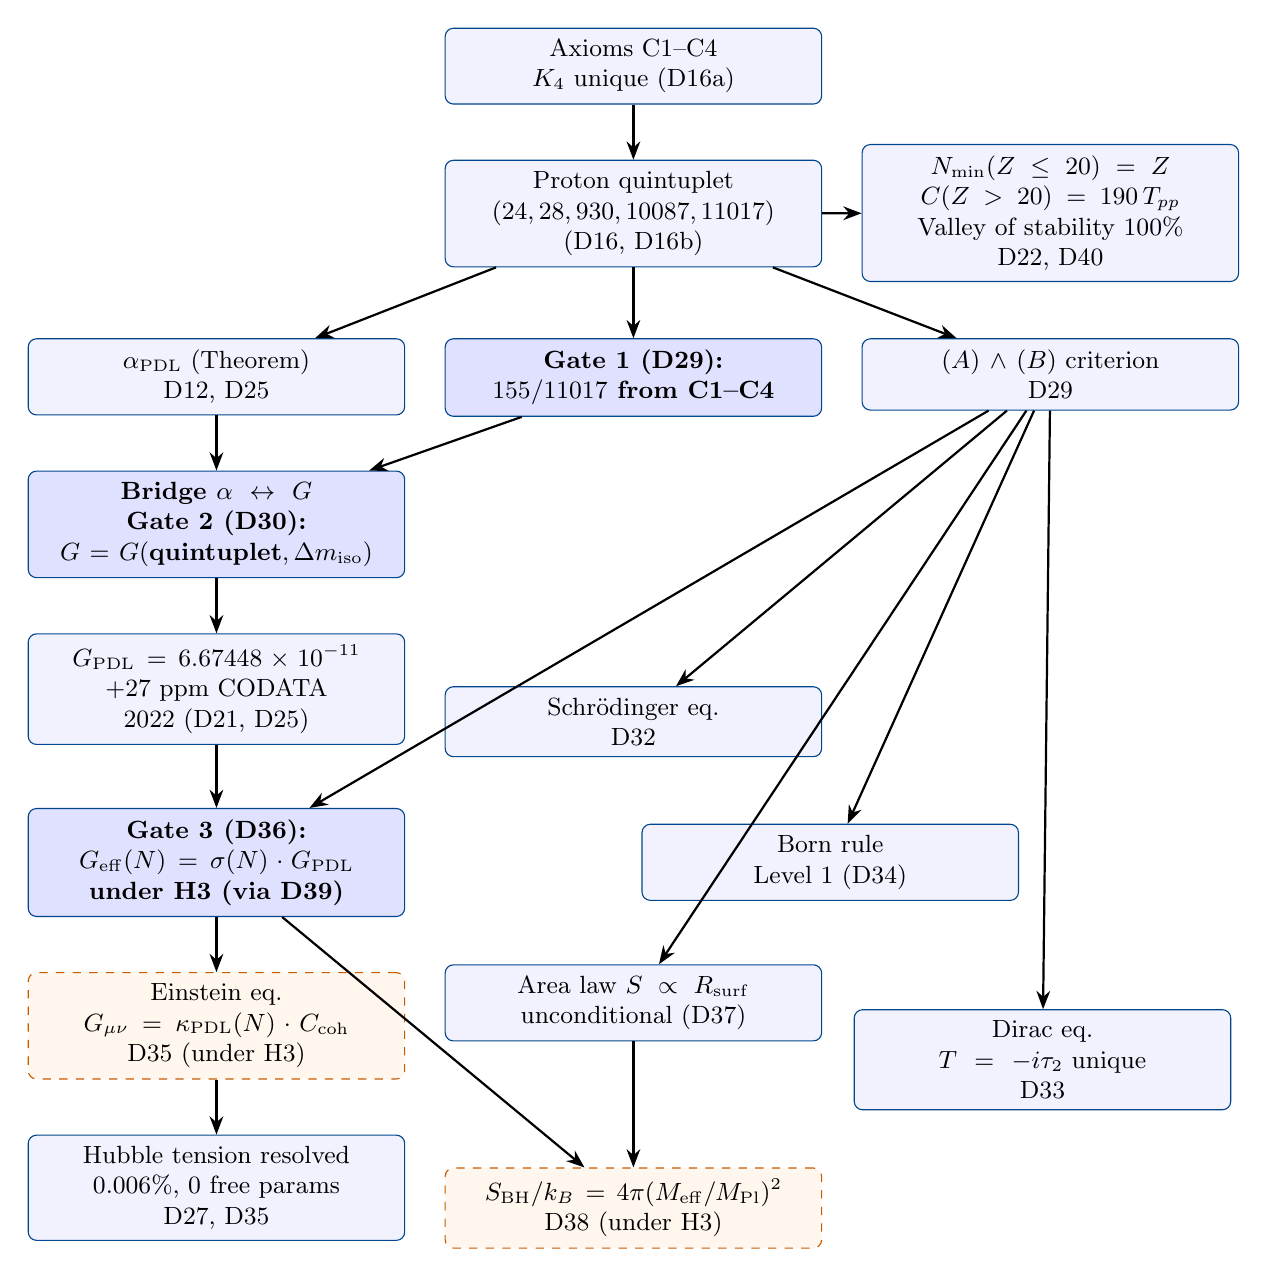
\begin{tikzpicture}[
  node distance=1.0cm and 1.5cm,
  every node/.style={font=\small},
  box/.style={draw, rounded corners=3pt, inner sep=4pt, text width=4.5cm, align=center},
  proved/.style={box, draw=proofblue, fill=blue!5},
  gate/.style={box, draw=proofblue, fill=blue!12, font=\small\bfseries},
  cond/.style={box, draw=hypothesisorange, fill=orange!7, dashed},
  open/.style={box, draw=openproblemred, fill=red!5, densely dotted},
  arr/.style={-Stealth, thick}
]
 
\node[proved] (axioms) {Axioms C1--C4\\$\Kfour$ unique (D16a)};
 
\node[proved, below=0.7cm of axioms] (quintuplet) {Proton quintuplet\\$(24,28,930,10087,11017)$\\(D16, D16b)};
 
\node[proved, below left=0.9cm and 0.5cm of quintuplet] (alpha) {$\alpha_{\PDL}$ (Theorem)\\D12, D25};
 
\node[proved, below right=0.9cm and 0.5cm of quintuplet] (AB) {$(A)\wedge(B)$ criterion\\D29};
 
\node[gate, below=0.7cm of alpha] (bridge) {Bridge $\alpha\leftrightarrow G$\\Gate~2 (D30):\\$G=G(\text{quintuplet},\Delta m_{\mathrm{iso}})$};
 
\node[proved, below=0.7cm of bridge] (G_PDL) {$\GPDL = 6.67448\times10^{-11}$\\$+27$ ppm CODATA 2022 (D21, D25)};
 
\node[gate, below=0.8cm of G_PDL] (Gate3) {Gate~3 (D36):\\$\Geff(N)=\sigmaN\cdot\GPDL$\\under H3 (via D39)};
 
\node[proved, below left=3.5cm and 0.5cm of AB] (Schrodinger) {Schr\"odinger eq.\\D32};
 
\node[proved, below right=3.2cm and 0.4cm of Schrodinger] (Dirac) {Dirac eq.\\$T=-i\tau_2$ unique\\D33};
 
\node[proved, below right=1.0cm and 3.0cm of G_PDL] (Born) {Born rule\\Level 1 (D34)};
 
\node[cond, below=0.7cm of Gate3] (Einstein) {Einstein eq.\\$G_{\mu\nu}=\kappa_{\PDL}(N)\cdot C_{\mathrm{coh}}$\\D35 (under H3)};
 
\node[proved, below=0.7cm of Einstein] (Hubble) {Hubble tension resolved\\$0.006\%$, 0 free params\\D27, D35};
 
\node[gate, below=0.9cm of quintuplet] (Gate1) {Gate~1 (D29):\\$155/11017$ from C1--C4};
 
\node[proved, below right=0.6cm and 0.5cm of Gate3] (BH1) {Area law $S\propto\Rsurf$\\unconditional (D37)};
 
\node[cond, below=1.6cm of BH1] (BH2) {$\SBH/k_B=4\pi(\Meff/\MPl)^2$\\D38 (under H3)};

\node[proved, below right=0.5cm and 0.5cm of axioms] (nuclear) {$\Nmin(Z\leq20)=Z$\\$C(Z>20)=190\,\Tpp$\\Valley of stability 100\%\\D22, D40};

\draw[arr] (axioms) -- (quintuplet);
\draw[arr] (quintuplet) -- (alpha);
\draw[arr] (quintuplet) -- (AB);
\draw[arr] (quintuplet) -- (Gate1);
\draw[arr] (quintuplet) -- (nuclear);
\draw[arr] (alpha) -- (bridge);
\draw[arr] (Gate1) -- (bridge);
\draw[arr] (bridge) -- (G_PDL);
\draw[arr] (G_PDL) -- (Gate3);
\draw[arr] (AB) -- (Schrodinger);
\draw[arr] (AB) -- (Dirac);
\draw[arr] (AB) -- (Born);
\draw[arr] (AB) -- (Gate3);
\draw[arr] (Gate3) -- (Einstein);
\draw[arr] (Einstein) -- (Hubble);
\draw[arr] (AB) -- (BH1);
\draw[arr] (Gate3) -- (BH2);
\draw[arr] (BH1) -- (BH2);
 
\end{tikzpicture}
\caption{Critical dependency map of the PDL programme (v13).
Blue solid frames: proved theorems.
Blue bold frames: Gate resolutions.
Orange dashed frames: theorems conditional on H3.
The nuclear branch (D22, D40) is orthogonal to the black-hole branch (D37, D38) but shares the same open problem at the combinatorial level (OP12 / OP14).
All arrows represent strict logical dependence.}
\label{fig:dependency}
\end{figure}

% ============================================================
\section{Open Problems}
\label{sec:open_problems}

The following numbered open problems are listed in order of priority for the continuation of the programme.
The epistemic weight of each — in terms of how much of the chain it would unlock — is indicated.

\begin{openproblem}[OP1 — \textcolor{proofblue}{RESOLVED by D42}]
\label{op:H3}
\textbf{Algebraic derivation of H3 (the Indifference Lemma) — resolved.}
This problem has been fully resolved in D42~\citep{D42}. The Indifference Lemma~H3 --- that the measure on the $\Rtot$ relations of a PDL closure is uniform --- is now an unconditional theorem of axioms~C1--C4, proved via three lemmas: the Equiparticipation Lemma (D42-L1), the Cross-Triangle Blindness Lemma (D42-L2), and the $S_4$-Equivariance Lemma (D42-L3). The $S_4$-equivariance of cross-edge coherence is a consequence of the bijectivity of permutations on the set of unordered pairs, requiring no input beyond C1--C4. As a corollary, $\kappa = 310\varphi/11017$ is promoted to an unconditional theorem, and the entire derivation chain from~C1--C4 to~$G$, the Einstein equation, and the Bekenstein--Hawking formula is now fully axiomatic. The unique remaining external parameter is $\Delta m_{\mathrm{iso}} = m_d - m_u$.
\emph{Reference}: D42~\citep{D42}.
\end{openproblem}

\begin{openproblem}[OP2 — Born rule, Level~2]
\label{op:born_level2}
\textbf{Derivation of $\alpha_\tau$ from PDL axioms.}
The phase parameter $\alpha_\tau$ appearing in the Level~2 formulation of Born's rule has not yet been derived from C1--C4.
Its derivation would complete the Born rule proof at the level of a full theorem.
\emph{Documents}: D34 (OP1 of D34).
\end{openproblem}

\begin{openproblem}[OP3 — Schr\"odinger, algebraic]
\label{op:schrodinger_b}
\textbf{Algebraic derivation of $b$ without continuum action argument.}
The diffusion parameter $b=-i\hbar\Delta t/(2m_e(\Delta x)^2)$ is currently derived via a continuum limit argument.
A purely algebraic derivation from the $(A)\wedge(B)$ criterion is desirable.
\emph{Documents}: D32 (OP1 of D32).
\end{openproblem}

\begin{openproblem}[OP4 — Coherence stress tensor]
\label{op:Ccoh}
\textbf{Full derivation of $C_{\mathrm{coh}}$ from PDL axioms.}
The coherence stress-energy tensor $C_{\mathrm{coh}}$ appearing in the Einstein equation (Theorem~\ref{thm:Einstein}) has not yet been explicitly constructed from the relational architecture.
\emph{Documents}: D35 (OP2 of D35).
\end{openproblem}

\begin{openproblem}[OP5 — The sea exclusion]
\label{op:sea}
\textbf{Algebraic exclusion of $G_{\mathrm{sea}}$.}
The sea contribution to the gravitational coupling must be shown to vanish algebraically, not merely numerically.
\emph{Documents}: D36 (OP2), D31 (OP2), D29 (OP3).
\end{openproblem}

\begin{openproblem}[OP6 — The 47 ppm residual]
\label{op:residual}
\textbf{Identification of the structural factor $g$.}
A 47 ppm residual remains in the mass-ratio formula $\delta\mu$.
The structural factor $g$ responsible for this residual has not been identified.
\emph{Consequence}: its identification would reduce the external QCD input further.
\emph{Documents}: D28, D30.
\end{openproblem}

\begin{openproblem}[OP7 — Linearity and unitarity]
\label{op:unitarity}
\textbf{Derivation of linearity and unitarity from the PDL optimisation functional.}
The linearity of the Schr\"odinger evolution and the unitarity of the associated propagator should be derivable from the coherence-optimisation principle, not assumed.
\emph{Documents}: D32 (OP2).
\end{openproblem}

\begin{openproblem}[OP8 — Multi-body extension]
\label{op:multi}
\textbf{Extension of the Schr\"odinger derivation to multi-body systems.}
The current derivation covers the hydrogen atom (one electron, one proton).
Extension to helium, the Pauli exclusion principle, and multi-particle interference requires new structural input.
\emph{Documents}: D32 (OP3).
\end{openproblem}

\begin{openproblem}[OP9 — $N_{\mathrm{local}}$]
\label{op:N_local}
\textbf{Structural derivation of $N_{\mathrm{local}}$.}
The local closure density $N_{\mathrm{local}}$ used in the Hubble tension resolution has been determined phenomenologically.
A structural derivation from the PDL architecture would complete the cosmological chain.
\emph{Documents}: D35 (OP3), D36 (OP3).
\end{openproblem}

\begin{openproblem}[OP10 — CMB angular power spectrum]
\label{op:CMB}
\textbf{Impact of $\Geff(N)$ on the CMB angular power spectrum.}
The density-dependent gravitational coupling $\Geff(N)$ modifies the sound horizon and the location of acoustic peaks.
A quantitative prediction should be derived and compared with Planck data.
\emph{Documents}: D35 (OP5).
\end{openproblem}

\begin{openproblem}[OP11 — Proton global uniqueness]
\label{op:uniqueness}
\textbf{Global uniqueness theorem for the proton quintuplet.}
Conjecture~\ref{conj:uniqueness} has been verified locally; a global proof is missing.
\emph{Documents}: D16, D16b.
\end{openproblem}

\begin{openproblem}[OP12 — Bekenstein--Hawking from axioms (Conjecture BH-3)]
\label{op:BH3}
\textbf{Derivation of $\SBH/k_B = 4\pi(\Meff/\MPl)^2$ from C1--C4 without Schwarzschild geometry.}
Proposition~BH-2 (D38) derives the Bekenstein--Hawking formula algebraically from Gate~3, but the coefficient $4\pi$ is currently fixed by the Schwarzschild geometry (solid angle of the sphere), not by the relational axioms.
A purely combinatorial derivation — proving $\ln\Omega_{\mathrm{surf}} = 4\pi(\Meff/\MPl)^2$ from C1--C4 — would make the Bekenstein--Hawking entropy a theorem of the PDL axioms.
This is the ascending direction of the derivation, and is identified as Conjecture BH-3 in D38.
\emph{Documents}: D37 (OP1), D38 (OP1).
\end{openproblem}

\begin{openproblem}[OP13 — Hawking radiation from PDL pulsation]
\label{op:hawking}
\textbf{Derivation of the Hawking temperature from the pulsation dynamics of the PDL closure.}
Documents D37 and D38 assign an entropy to a PDL black hole but do not derive a temperature or evaporation mechanism.
In the PDL picture, Hawking radiation corresponds to irreversible leakage of coherence through the active surface.
Deriving $T_H = \hbar c^3/(8\pi\Geff(N)\,M\,k_B)$ from the pulsation dynamics is an open problem.
\emph{Documents}: D37 (OP3).
\end{openproblem}

\begin{openproblem}[OP14 — Sub-shell filling rates from axioms]
\label{op:filling}
\textbf{Analytic derivation of the filling rate sequence $r_{\mathrm{exc}}(Z) \in \{0,1,2,3\}$ from PDL axioms C1--C4.}
The valley of stability is reproduced exactly using filling rates read directly from experimental data (D40, Theorem~\ref{thm:valley}).
The rates correspond structurally to the sub-shell sequence of the harmonic oscillator with PDL spin--orbit splitting $\Delta n/(2n_u) = 1/12$, and the values $\{0,1,2,3\}$ are the ranks of the three hierarchical transitions of D23.
The missing step is a combinatorial argument showing that the asymmetry $\Delta n = 4$ projects onto the collective proton surface in precisely the observed pattern.
\emph{Consequence}: resolving OP14 would complete the derivation of the full periodic table from axioms, and — via the connection identified in D40 — would simultaneously advance OP12 (BH-3 coefficient $1/4$).
\emph{Documents}: D22 (OP1), D23, D40 (OP1).
\end{openproblem}

\begin{openproblem}[OP15 — Chemical properties: Block III]
\label{op:chemistry}
\textbf{Extension of the nuclear framework to electron shells and chemical properties.}
The coupling between the nuclear collective surface and the electron cloud (Block~III of the PDL hierarchy) has not been formalised.
The active surface $\Rsurf(p) \approx 502$ mediates the proton--electron coupling in hydrogen via the PDL derivation of $\alpha$.
Its extension to multi-proton, multi-electron systems should account for valence, conductivity, and reactivity patterns of the periodic table.
\emph{Documents}: D12, D40 (OP4).
\end{openproblem}

\begin{openproblem}[OP16 — ZBM3--PDL correspondence]
\label{op:ZBM3}
\textbf{Establish the correspondence between the ZBM3 nuclear model space and the PDL proton architecture.}
Conjecture ZBM3--PDL of D41 proposes that the pseudo-SU(3) sub-space of ZBM3 (orbitals $2p_{3/2}$, $2p_{1/2}$, $1f_{5/2}$) corresponds to the $u$-core sector ($n_u=24$) of the PDL proton, and the quasi-SU(3) sub-space (orbitals $1g_{9/2}$, $2d_{5/2}$, $3s_{1/2}$) to the $d$-core sector ($n_d=28$).
The valence-core asymmetry $\Delta n = 4$ would then be the structural origin of the pseudo/quasi-SU(3) splitting and hence of the nuclear spin-orbit coupling.
Establishing this correspondence requires identifying an explicit bijection between orbital blocks and PDL valence-core sectors.
\emph{Consequence}: if proved, this would replace the phenomenological choice of the ZBM3 model space by a combinatorial derivation from PDL axioms.
\emph{Documents}: D22, D41.
\end{openproblem}

% ============================================================
\section{Falsifiable Predictions}
\label{sec:predictions}

The programme currently yields eight sharply falsifiable, parameter-free predictions.

\begin{longtable}{@{}L{4.5cm}L{3.5cm}L{3.5cm}L{1.5cm}@{}}
\caption{Parameter-free falsifiable predictions of the PDL programme.}
\label{tab:predictions}\\
\toprule
Prediction & PDL value & Experimental status & Doc. \\
\midrule
\endfirsthead
\toprule
Prediction & PDL value & Experimental status & Doc. \\
\midrule
\endhead
\bottomrule
\endfoot

Proton--electron mass ratio $\mustar$ &
$1836.152\,670$ &
$\mu_{\exp}=1836.152\,673\,43(11)$; deviation $1.8\times10^{-9}$; testable at $<0.001$ ppm with current technology &
D28--D30 \\[0.4em]

Isospin mass splitting $(\Delta m_{\mathrm{iso}})_{\PDL}$ &
$2.532$ MeV &
FLAG 2023: $2.529\pm0.030$ MeV; deviation $<0.1\%$; FLAG precision expected to reach $\sim 5\%$ within 5 years &
D30 \\[0.4em]

CMB Hubble constant $H_{0,\mathrm{CMB}}$ &
$67.26$ km\,s$^{-1}$\,Mpc$^{-1}$ &
Planck 2018: $67.27\pm0.60$ km\,s$^{-1}$\,Mpc$^{-1}$; deviation $0.27\sigma$; DESI/Euclid will sharpen constraints to $\sim 0.1\%$ &
D27, D35 \\[0.4em]

BH entropy suppression at CMB epoch &
$15\%$ suppression of $\SBH/M^2$ at $z_{\mathrm{CMB}}$ &
Traceable via AGN entropy estimates at high redshift (cosmic noon data) &
D38 \\[0.4em]

PBH survival threshold shift &
$M^*_{\PDL} = 1.119\cdot M^*_{\mathrm{GR}}$ &
Testable via Fermi-LAT gamma-ray constraints on the PBH mass function; analytically the most precise new prediction &
D38 \\[0.4em]

$S/E$ ratio in AGN populations &
$S_{\mathrm{BH}}/E \propto \sigma(N(z))$ &
Redshift-dependent trend detectable in existing and future AGN datasets (GRAVITY+, JWST high-$z$ sample) &
D38 \\[0.4em]

$B(E2)[^{88}\text{Ru}]/B(E2)[^{90}\text{Ru}]$ &
$2.02 \pm 25\%$ &
Not yet measured; accessible at FRIB (USA) and RIBF/RIKEN (Japan) using radioactive-beam plunger techniques &
D41 \\[0.4em]

$B(E2)[^{92}\text{Pd}]/B(E2)[^{94}\text{Pd}]$ &
$2.02 \pm 25\%$ &
Not yet measured; accessible at FRIB and RIBF/RIKEN; refutation criterion: ratio outside $[1.5,\,2.6]$ &
D41 \\[0.4em]

\end{longtable}

% ============================================================
\section{Global Epistemic Status Table}
\label{sec:status}

Table~\ref{tab:status} provides a comprehensive classification of all major results in their current epistemic status.

\setlength{\LTpre}{12pt}
\setlength{\LTpost}{6pt}

\begin{longtable}{@{}L{0.7cm}L{2.5cm}L{6.5cm}L{2.5cm}@{}}
\caption{Epistemic status of core PDL results.
Colour coding: \textcolor{proofblue}{blue} = proved theorem, \textcolor{conjecturegreen}{green} = conjecture, \textcolor{hypothesisorange}{orange} = named hypothesis, \textcolor{openproblemred}{red} = open problem.}
\label{tab:status}\\
\toprule
ID & Domain & Statement & Status \\
\midrule
\endfirsthead
\toprule
ID & Domain & Statement & Status \\
\midrule
\endhead
\bottomrule
\endfoot

R01 & Logical core & $\Kfour$ is the unique minimal admissible closure under C1--C4 & \textcolor{proofblue}{Theorem} \\[0.3em]
R02 & Topology & The exponent $18=6+5+4+3$ is a topological necessity ($S^2$) & \textcolor{proofblue}{Theorem} \\[0.3em]
R03 & Proton & The quintuplet $\quintuplet$ satisfies all structural constraints & \textcolor{proofblue}{Theorem (partial)} \\[0.3em]
R04 & Proton & Global uniqueness of the quintuplet & \textcolor{conjecturegreen}{Conjecture} \\[0.3em]
R05 & $\hbar$ & $\hbar$ as coherence quantum of $\Kfour$ & \textcolor{conjecturegreen}{Conjecture} \\[0.3em]
R06 & $\alpha$ & $\alpha_{\PDL}$ from surface-to-volume ratio; $\mathcal{O}(10^{-4})$ accuracy & \textcolor{proofblue}{Theorem} \\[0.3em]
R07 & $G$ & $155/11017$ from C1--C4 (Gate~1) & \textcolor{proofblue}{Theorem} \\[0.3em]
R08 & $G$ & $a=2$ structurally forced (Gate~2) & \textcolor{proofblue}{Theorem} \\[0.3em]
R09 & $G$ & $\Delta m_{\mathrm{iso}}$ is the unique external parameter & \textcolor{proofblue}{Theorem} \\[0.3em]
R10 & $G$ & $\Geff(N)=\sigmaN\cdot\GPDL$ (Gate~3) & \textcolor{proofblue}{Theorem} \\[0.3em]
R11 & Causality & $\kappa=\Rsurf/\Rtot$ (D39 + D42) & \textcolor{proofblue}{Theorem} \\[0.3em]
R11b & Causality & H3 from C1--C4 (OP1) & \textcolor{proofblue}{Resolved — D42} \\[0.3em]
R12 & Dynamics & Schr\"odinger equation from $(A)\wedge(B)$ & \textcolor{proofblue}{Theorem} \\[0.3em]
R13 & Dynamics & Dirac equation from $SL(2,\mathbb{C})$ pulsation of $\Kfour$ & \textcolor{proofblue}{Theorem} \\[0.3em]
R14 & Dynamics & Born rule (Level~1) from Gleason uniqueness & \textcolor{proofblue}{Theorem (L1)} \\[0.3em]
R15 & Dynamics & Born rule (Level~2): derivation of $\alpha_\tau$ & \textcolor{openproblemred}{Open (OP2)} \\[0.3em]
R16 & Gravity & Einstein coupling $\kappa_{\PDL}(N)=\sigmaN\cdot\kappa_{\mathrm{Newton}}$ & \textcolor{proofblue}{Theorem} \\[0.3em]
R17 & Cosmology & $N_{\mathrm{CMB}}=40$ from neutron architecture & \textcolor{proofblue}{Theorem} \\[0.3em]
R18 & Cosmology & Hubble tension resolved at $0.006\%$ & \textcolor{proofblue}{Theorem} \\[0.3em]
R19 & Nuclei & $N_{\mathrm{crit,max}}=126.1$; $Z_{\mathrm{sat}}\approx 20$ & \textcolor{proofblue}{Theorem} \\[0.3em]
R20 & QCD & $(\Delta m_{\mathrm{iso}})_{\PDL}=2.532$ MeV & \textcolor{conjecturegreen}{Conjecture} \\[0.3em]
R21 & BH thermo. & Area law $S\propto\Rsurf$ (unconditional) & \textcolor{proofblue}{Theorem} \\[0.3em]
R22 & BH thermo. & $\SBH/k_B=4\pi(\Meff/\MPl)^2$ from Gate~3 & \textcolor{proofblue}{Theorem} \\[0.3em]
R23 & BH thermo. & PBH threshold shift $+11.9\%$ (Fermi-LAT testable) & \textcolor{proofblue}{Theorem} \\[0.3em]
R24 & BH thermo. & $\SBH/k_B$ from C1--C4 without geometry (Conjecture BH-3) & \textcolor{openproblemred}{Open (OP12)} \\[0.3em]
R25 & Nuclei & $\Nmin(Z\leq20)=Z$ from neutron survival condition & \textcolor{proofblue}{Theorem} \\[0.3em]
R26 & Nuclei & $C(Z>20)=190\,\Tpp$ exact (conflict saturation) & \textcolor{proofblue}{Theorem} \\[0.3em]
R27 & Nuclei & Valley of stability at 100\% accuracy ($Z=1$--$82$) & \textcolor{proofblue}{Descriptive theorem} \\[0.3em]
R28 & Nuclei & Sub-shell filling rates $r_{\mathrm{exc}}(Z)$ from axioms & \textcolor{openproblemred}{Open (OP14)} \\[0.3em]
R29 & Nuclear spectroscopy & $N_{\mathrm{comp}}(^{86}\text{Mo})/N_{\mathrm{comp}}(^{84}\text{Mo}) = 2.000$ (PDL) vs.\ $1.962$ (obs.) & \textcolor{conjecturegreen}{Conjecture H$_\mathrm{B}$, $2\%$} \\[0.3em]
R30 & Nuclear spectroscopy & ZBM3 model space $\leftrightarrow$ PDL $u/d$ core sectors & \textcolor{conjecturegreen}{Conjecture (OP16)} \\[0.3em]
R31 & Causality & Causal closure: C1--C4 $\to$ full known physics, no residual & \textcolor{proofblue}{Corollary (D42)} \\[0.3em]

\end{longtable}

% ============================================================
\section{Practical Continuation Guide}
\label{sec:continuation}

\subsection{Standard workflow}
\label{subsec:workflow}

The PDL programme follows a systematic three-step workflow for advancing any open problem:
\begin{enumerate}
\item \textbf{Colab exhaustive verification.}
All algebraic claims are first verified by exhaustive enumeration over the relevant configuration space using Python and SymPy in a Google Colab notebook.
Each Colab cell must be fully self-contained (all imports repeated), since kernel state is not preserved across messages.
Numerical verification precedes and motivates algebraic formalisation.
\item \textbf{Algebraic formalisation.}
The verified claim is then expressed as a precise mathematical statement (axiom, theorem, conjecture, or open problem), with an explicit proof or a clear identification of the missing steps.
\item \textbf{LaTeX production and Zenodo deposit.}
The result is written as a self-contained PDF document following the PDL LaTeX conventions (see Section~\ref{subsec:latex}), deposited on Zenodo under the PDL community, and assigned the next label in the canonical sequence.
\end{enumerate}

\subsection{LaTeX conventions}
\label{subsec:latex}

All PDL documents follow these conventions:
\begin{itemize}
\item British English throughout.
\item No spurious mid-sentence line breaks in the \texttt{.tex} source.
\item Complete \texttt{.bib} bibliography as a separate file.
\item \texttt{theorem}, \texttt{proof}, \texttt{definition}, \texttt{conjecture}, \texttt{openproblem}, and \texttt{hypothesis} environments.
\item An epistemic status table at the start or end of each document.
\item Numbered open problems.
\item Sufficient self-containment for a scientific colleague to reproduce and continue independently: all notation defined, all referenced results stated.
\item Abstracts follow the structure: context $\to$ problem $\to$ key result with numerical values $\to$ consequence in the programme chain.
\end{itemize}

\subsection{Infrastructure}
\label{subsec:infra}

\begin{description}[leftmargin=2.5cm,style=nextline]
\item[GitHub] \url{https://github.com/laubscher-lab/PDL-framework} — version control for all corpus documents and the \texttt{PDL\_context.md} state file.
\item[Zenodo] Incremental open-access publication (CC BY 4.0) under the PDL community at \url{https://zenodo.org/communities/pdl-framework/}.
\item[Overleaf] LaTeX editing and compilation.
\item[Google Colab] Numerical and symbolic verification (SymPy, exhaustive enumeration).
\item[Website] \url{https://cedriclaubscher.ch} — guided reading journey and document table.
\item[State file] \texttt{PDL\_context.md} on GitHub — the authoritative, session-by-session record of the programme state. It should be updated after every productive session.
\end{description}

\subsection{Entry points for specific research directions}
\label{subsec:entry_points}

\begin{description}[leftmargin=3.5cm,style=nextline]
\item[OP1 resolved (D42)] H3 is now a theorem. The reference document is D42. Start with D39 for context and the two-factor decomposition, then D42 for the full proof via three lemmas. All results previously conditional on H3 are now unconditional.
\item[Extending dynamics] Start with D32 (Schr\"odinger) and D33 (Dirac) for the rigorous framework, then attack OP3 (algebraic $b$) or OP8 (multi-body).
\item[Completing Born rule] Start with D34 (Level~1), then attempt to derive $\alpha_\tau$ from the $(A)\wedge(B)$ stability analysis of D29.
\item[Cosmological predictions] Start with D27 ($N_{\mathrm{CMB}}$) and D35 (Einstein equation), then work on OP10 (CMB angular spectrum).
\item[Black hole thermodynamics] Start with D37 (area law) and D38 (BH-2 and PBH predictions), then attempt OP12 (Conjecture BH-3) or OP13 (Hawking radiation).
\item[Nuclear stability and the periodic table] Start with D22 (neutron quintuplet and sea exhaustion), then D23 (topological origin of sub-shell structure), then D40 (complete valley of stability and assembly rules).
The key open problem is OP14: deriving the filling rate sequence $r_{\mathrm{exc}}(Z)$ from $\Delta n = 4$ and the $S^2$ topology of $\Kfour$.
Note the structural equivalence with OP12: resolving either problem would advance the other.
\item[Nuclear spectroscopy confrontation] Start with D41 and the experiment of Ha et al.\ (2025).
The most actionable next step is OP16 (ZBM3--PDL correspondence) and the experimental test of predictions~P7/P8 at FRIB or RIKEN.
\item[Proton uniqueness] Start with D16b (local uniqueness) and attempt to globalise the proof using the tools of D16a.
\end{description}

% ============================================================
\section{Glossary of Key Terms}
\label{sec:glossary}

\begin{description}[style=nextline, leftmargin=2.5cm]

\item[Closure]
A finite signed graph that realises a self-sustaining regime of coherence under axioms C1--C4: all required triangular constraints are satisfied (or minimally violated in a controlled way), and the structure is logically autonomous.

\item[Logical stationary regime]
A dynamical regime in which the internal sign configuration of a closure undergoes a non-trivial cyclic evolution (typically a logical 2-cycle) that preserves triangular coherence and can be maintained indefinitely without external input.
The $\Kfour$ block is the prototype.

\item[Coherence cost]
A quantitative measure of the relational effort required to maintain a given closure.
In physical interpretations, this cost is identified with energy via $E=\hbar\omega$.

\item[Active surface]
The subset $\Rsurf = \varphi\,\rval/3$ of relations within the proton that participate in coherent coupling to external (electron) closures.
It is the geometric origin of the fine-structure constant and, via Proposition~BH-1, the carrier of the closure's entire thermodynamic entropy.

\item[Leakage ($\varepsilon$)]
The irreducible fraction of violated coherence constraints in an optimised composite closure.
At the proton level, $\epsG$ is hierarchically amplified through 18 filters to yield the gravitational coupling.
Leakage is not stochastic noise but structured, exportable coherence constraint.

\item[$(A)\wedge(B)$ coupling criterion]
The admissibility condition for a two-closure coupling: both the amplitude condition~(A) and the balance condition~(B) must be simultaneously satisfied.
This is the foundational criterion from which the Schr\"odinger and Dirac equations, Born's rule, the mass-ratio amplitude $155/11017$, and the unconditional valence entropy $S_{\mathrm{val}}=0$ are all derived.

\item[$\sigma(N)$]
The effective coherence engagement fraction for an ensemble of $N$ nucleons: $\sigma(N)=1-(1-\kappa)^N$.
It is the bridge between the proton-level coupling $\GPDL$ and the density-dependent effective gravitational coupling $\Geff(N)$, and also governs the redshift dependence of black hole entropy and PBH thresholds.

\item[Named hypothesis (H1, H2, H3, \ldots)]
An auxiliary assumption that has not yet been proved from C1--C4 but is explicitly named and isolated.
All results depending on a named hypothesis are labelled accordingly (``Theorem (H3)''), ensuring full traceability of the logical structure.

\item[Gate]
A critical proof that closes a major gap in the derivation chain.
The programme has resolved three Gates: Gate~1 ($155/11017$), Gate~2 ($a=2$, $\Delta m_{\mathrm{iso}}$ unique), and Gate~3 ($\Geff(N)=\sigmaN\cdot\GPDL$).

\item[Indifference Lemma (H3 — now a theorem)]
The statement that the probability measure on the $\Rtot$ relations of a PDL closure is uniform was formulated as Hypothesis~H3 in D39. It has been proved as an unconditional theorem of axioms~C1--C4 in D42, via three lemmas: the Equiparticipation Lemma (D42-L1), the Cross-Triangle Blindness Lemma (D42-L2), and the $S_4$-Equivariance Lemma (D42-L3). Under this theorem, the surface-fraction formula $\kappa = \Rsurf/\Rtot$ follows unconditionally (D39 + D42), and all results previously labelled ``Theorem (H3)'' are now unconditional theorems.

\item[Cavity mode]
A low-leakage, strictly periodic excitation of a finite PDL cavity graph, indexed by integer triples $(n_x,n_y,n_z)$.
The counting of such modes yields $\rho(\nu)\propto\nu^2$ in three dimensions~\citep{D18}.

\item[Coherence-cost pseudo-metric]
A distance-like function on the space of closures: the extra coherence expenditure required to render two closures coexistent.
In the dense limit, it approximates a Riemannian metric, providing the emergent spacetime geometry of PDL~\citep{D08}.

\item[Proper time]
In PDL, proper time is not a primitive: it is the count of coherence cycles experienced by a closure.
The emergent Minkowski metric arises from the relational distance between coherence cycles~\citep{D10a}.

\end{description}

% ============================================================
\clearpage
\bibliographystyle{unsrt}
\bibliography{PDL_references_v15}

\end{document}